\section{Grundlagen}
	
	\subsection{iTool3}
	
	iTool3 ist eine auf dem CakePHP 3.3 - Framework basierende eCommerce Software Lösung zur Steuerung von Produktsortimenten auf verschiedenen Marktplätzen mit dem Ziel, den
	Vertriebsprozess zu automatisieren. Es ermöglicht dem Benutzer über eine einzelne Benutzeroberfläche Produkte auf Marktplätzen wie eBay, Amazon oder einem Magento Store
	zu verwalten. Produkte können dabei händisch erstellt oder aus bestehenden Datenquellen in die Software	eingepflegt werden. Im Anschluss ist es möglich diese Produkte auf einem oder mehreren Marktplätzen anzubieten. Die Verwaltung und Abwicklung der eingehenden Bestellungen läuft dabei komplett über das iTool.
	Da für jeden Marktplatz unterschiedliche Daten benötigt werden um auf ihm erfolgreich zu verkaufen, können für jedes Produkt unterschiedliche Attribute mit wiederum unterschiedlichen Werten angelegt werden. Die Produktverwaltung der Software folgt daher dem Entity-Attribute-Value Modell.
	
	
	\subsubsection{Verkäufer und Benutzer}
	
	Es wird unterschieden zwischen Verkäufern (Core-Seller) und Benutzern (Core-User). Ein Verkäufer ist z.B. "Markisenshop 2000". Diesem Verkäufer werden Benutzer zugeordnet, die mit mehr oder weniger Rechten ausgestattet, die Produkte z.B. nur einsehen können oder Kontrolle über die gesamte Produkt- und Bestellverwaltung haben.\\
	\begin{minipage}{\linewidth}
		\vspace{1em}
		\centering
		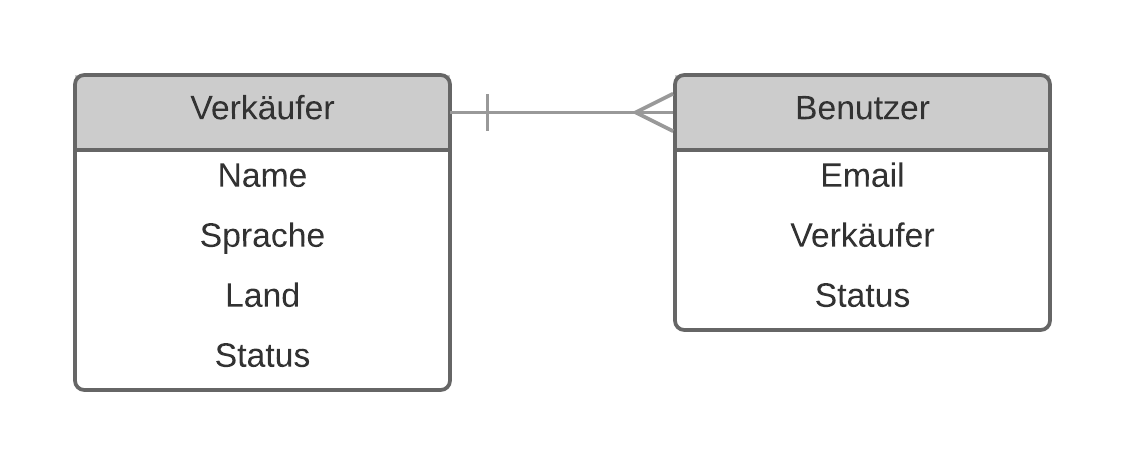
\includegraphics[width=0.6\linewidth]{img/ERD_Seller_User_complete}
		\captionof{figure}[ERD]{ER-Diagramm: Verkäufer - Benutzer}
		\label{fig:header}
		\vspace{1em}
	\end{minipage}
	
	Benutzerdaten werden in der Tabelle \texttt{core\_users} gespeichert, Verkäuferdaten in \texttt{core\_sellers}.

	 
	
	\subsubsection{Produktverwaltung}
	
	Die Produktverwaltung ist aufgeteilt in Produkte und Kategorien. \textbf{Produkte} besitzen Attribute wie Titel, Preis, Beschreibung etc. die für jeden Marktplatz auf denen diese angeboten werden sollen unterschiedlich ausfallen können. Es kann gewählt werden ob ein Produkt auf einem bestimmten Marktplatz angeboten werden soll oder nicht. Ein Produkt kann dabei mehreren \textbf{Kategorien} zugeordnet sein.\\
	\begin{minipage}{\linewidth}
		\vspace{1em}
		\centering
		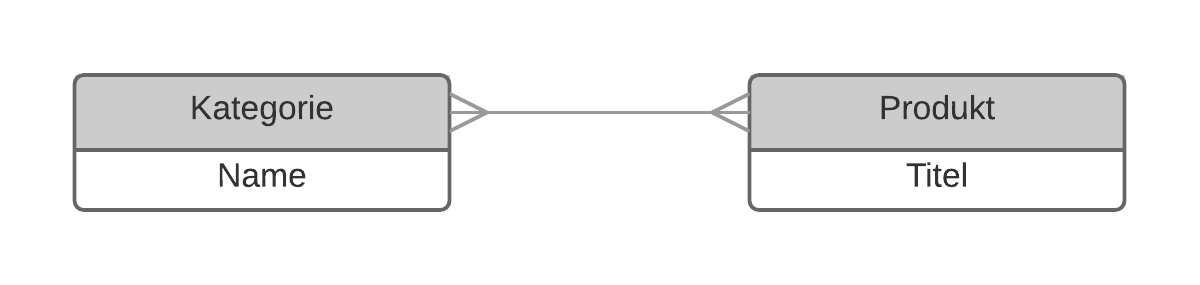
\includegraphics[width=0.6\linewidth]{img/ERD_Category_Product}
		\captionof{figure}[ERD]{ER-Diagramm: Kategorie - Produkt}
		\label{fig:header}
		\vspace{1em}
	\end{minipage}
	Eine Kind-Kategorie hat jeweils genau eine Eltern-Kategorie. Eine Eltern-Kategorie kann aber mehrere Kinder haben. Produkte sind genau einem Verkäufer zugeordnet. \\
	\begin{minipage}{\linewidth}
		\vspace{1em}
		\centering
		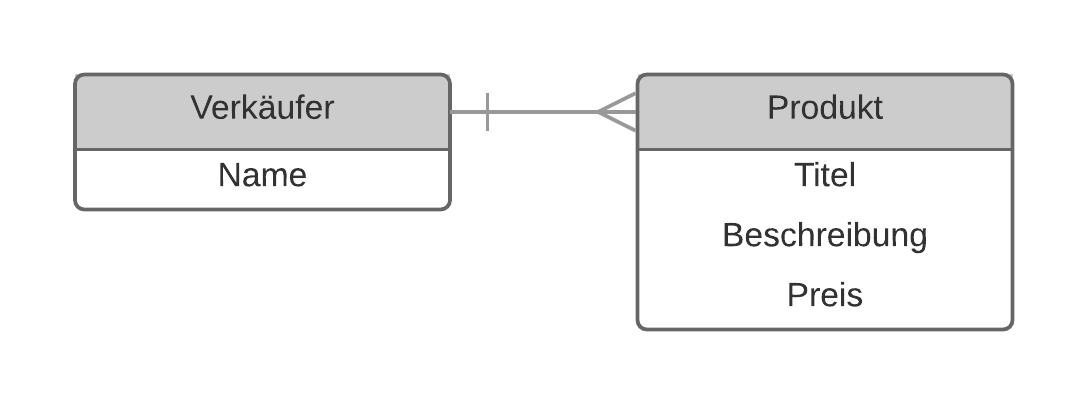
\includegraphics[width=0.6\linewidth]{img/ERD_Seller_Product}
		\captionof{figure}[ERD]{ER-Diagramm: Verkäufer - Benutzer}
		\label{fig:header}
		\vspace{1em}
	\end{minipage}
	
	Alle Produktdaten sind in der Tabelle \texttt{core\_products} und den damit verknüpften Tabellen hinterlegt.
	
	\subsubsection{Dashboard}
	
	Auf dem Dashboard werden Informationen über die Anzahl der insgesamt eingegangenen Bestellungen, den durchschnittlichen Bestellwert, die Gesamtzahl der Kunden, den insgesamt erwirtschafteten Umsatz, eine Übersicht der zuletzt eingegangenen Bestellungen sowie eine graphische Übersicht der während eines Jahres erwirtschafteten Umsätze angezeigt. 
	
	\subsection{Der BMECat}
	
	Der BMECat ist ein vom 'Bundesverband Materialwirtschaft, Einkauf und Logistik e.V' in Zusammenarbeit mit dem 'eBusiness Standardization Committee' entwickelter XML
	Standard mit dem Ziel den Austausch von Produktkatalogen zwischen Lieferanten und beschaffenden Organisationen zu standardisieren und somit zu vereinfachen.\footnote{BMECat V1.2 Spezifikation, Seite 5}. 
	
	\subsubsection{Terminologie}
	Ein \textbf{Produktkatalog} ist die Menge aller benötigten Daten, welche vom katalogerzeugenden Unternehmen an das katalogempfangende Unternehmen übermittelt werden sollen.\\
	Ein \textbf{Katalogdokument} ist eine XML-Datei, in der der Produktkatalog im BMECat-Format gespeichert und zum Katalogemfänger übermittelt wird.\\
	Eine \textbf{Kataloggruppe} ist ein Datenbereich, der eine Gruppe definiert, welcher gleichartige Artikel zugeordnet werden können. Diese wird im BMEcat-Format durch das Element \texttt{\textbf{CATALOG\_STRUCTURE}} abgebildet.\\
	Ein \textbf{Kataloggruppensystem} ist ein hierarchischer Baum von verknüpften Kataloggruppen. Es wird
	im BMEcat-Format durch das Element \texttt{\textbf{CATALOG\_GROUP\_SYSTEM}} abgebildet.\footnote{BMECat V1.2 Spezifikation, Seite 7}
	
	\subsubsection{Transaktionen}
	Im BMECat wird zwischen den 3 verschiedenen Transaktionsarten
	\begin{itemize}[noitemsep]
	\item \texttt{\textbf{T\_NEW\_CATALOG}} - Übertragung eines neuen Produktkataloges
	\item \texttt{\textbf{T\_UPDATE\_PRODUCTS}} - Aktualisierung von Produktdaten
	\item \texttt{\textbf{T\_UPDATE\_PRICES}} - Aktualisierung von Preisinformationen
	\end{itemize} 
	unterschieden. Die Unterscheidung geschieht um die Größe eines Katalogdokumentes zu reduzieren. Es muss so z.B. nicht ein kompletter Produktkatalog übertragen werden, falls sich bei einem \(oder mehreren\) Artikel\(n\) der Preis ändert.
	
	\subsubsection{Aufbau}
	
	Ein BMECat-Dokument besteht aus einer Folge von KANN und MUSS Feldern, den dazugehörigen Datentypen und Feldlängen und ist folgendermaßen aufgebaut:
		
		\begin{enumerate}
		
			\item XML-Deklaration und Header-Bereich (mit Informationen über Kataloganbieter und Empfänger, Bezeichnung und Erstellungsdatum des Kataloges etc.  )
				\\Bsp. für einen Header:
			\begin{lstlisting}
			<HEADER>
			  <GENERATOR_INFO> Kann </GENERATOR_INFO>
			  <CATALOG> Muss </CATALOG>
			  <BUYER> Kann </BUYER>
			  <SUPPLIER> Muss </SUPPLIER>
			</HEADER>
			\end{lstlisting}
			Bsp. für XML Deklaration:
			\begin{lstlisting}
			<?xml version="1.0" encoding="UTF-8"?>
			<!DOCTYPE BMECAT SYSTEM "bmecat_new_catalog.dtd">
			<BMECAT version="1.2" xml:lang="de" xmlns="http://www.bmecat.org/bmecat/1.2/bmecat_new_catalog">
			\end{lstlisting}
			\item Produktgruppensystem (Baumstruktur der Produktgruppen mit den Attributwerten Root, Node und Leaf)
			\begin{lstlisting}
			<CATALOG_STRUCTURE type="root">
			   <GROUP_ID>1</GROUP_ID>
			   <GROUP_NAME>Katalog</GROUP_NAME>
			   <PARENT_ID>0</PARENT_ID>
			   <GROUP_ORDER>1</GROUP_ORDER>
			</CATALOG_STRUCTURE>
			  <CATALOG_STRUCTURE type="node">
			   <GROUP_ID>2</GROUP_ID>
			   <GROUP_NAME>Spiele &amp; Konsolen</GROUP_NAME>
			   <PARENT_ID>1</PARENT_ID>
			 </CATALOG_STRUCTURE>
			 <CATALOG_STRUCTURE type="leaf">
			   <GROUP_ID>7</GROUP_ID>
			   <GROUP_NAME>PlayStation 4</GROUP_NAME>
			   <PARENT_ID>2</PARENT_ID>
			 </CATALOG_STRUCTURE>
			\end{lstlisting}
			
			
			
			\item Artikel (mit Attributen und Werten)
			
			\begin{lstlisting}
			<ARTICLE mode="new">
			  <SUPPLIER_AID>9057320097280</SUPPLIER_AID>
			    <ARTICLE_DETAILS>
			      <DESCRIPTION_SHORT>GTA 5</DESCRIPTION_SHORT>
			      <DESCRIPTION_LONG>Das tolle neue Spiel</DESCRIPTION_LONG>
			      <EAN>87126723434</EAN>
				... weitere Attribute ...
			    </ARTICLE_DETAILS>
				...weitere Felder ...
			</ARTICLE>
			\end{lstlisting}
			
	
			\item Zuordnung der Artikel zu den Produktgruppen.
			\begin{lstlisting}
			<ARTICLE_TO_CATALOGGROUP_MAP>
			  <ART_ID>9057320097280</ART_ID>
			  <CATALOG_GROUP_ID>7</CATALOG_GROUP_ID>
			</ARTICLE_TO_CATALOGGROUP_MAP>
			\end{lstlisting}
		
		\end{enumerate}
		
	--- Übersicht der im BMECat verwendeten Datentypen --- noch einfügen ---
	
	Im folgenden Abschnitt wird jeder Teilbereich mit seinen Unterelementen, wie sie in vorliegender Arbeit verwandt wurden, graphisch dargestellt und kurz erläutert. Rot hervorgehoben sind jeweils die MUSS-Felder, welche zwingend in einem gültigen BMECat Dokument vorkommen müssen, grün die KANN-Felder. Ein Plus \(+\) Zeichen hinter dem Elementnamen indiziert, dass dieses Element mehrfach an dieser Stelle vorkommen kann, jedoch mindestens einmal. Ein Asterisk \(*\) zeigt an, dass dieses Element einmal, mehrfach oder nicht vorkommen kann.  
	
	\textbf{\underline{Header}}\\
	Im Header werden allgemeine Informationen über das Katalogdokument hinterlegt und Default Werte gesetzt. Das Element \texttt{\textbf{CATALOG}} enthält dabei Informationen zur Identifikation und Beschreibung des Produktkataloges, wie z.B. die Katalog Id, die Katalogversion oder die für das Dokument geltende Sprache sowie Elemente zum setzten von Standard-Werten wie z.B. die für das Katalogdokument geltende Währungsangabe \footnote{BMECat V 1.2 Spezifikation, Seite 27,29} 
	
	\begin{minipage}{\linewidth}
		\vspace{1em}
		\centering
		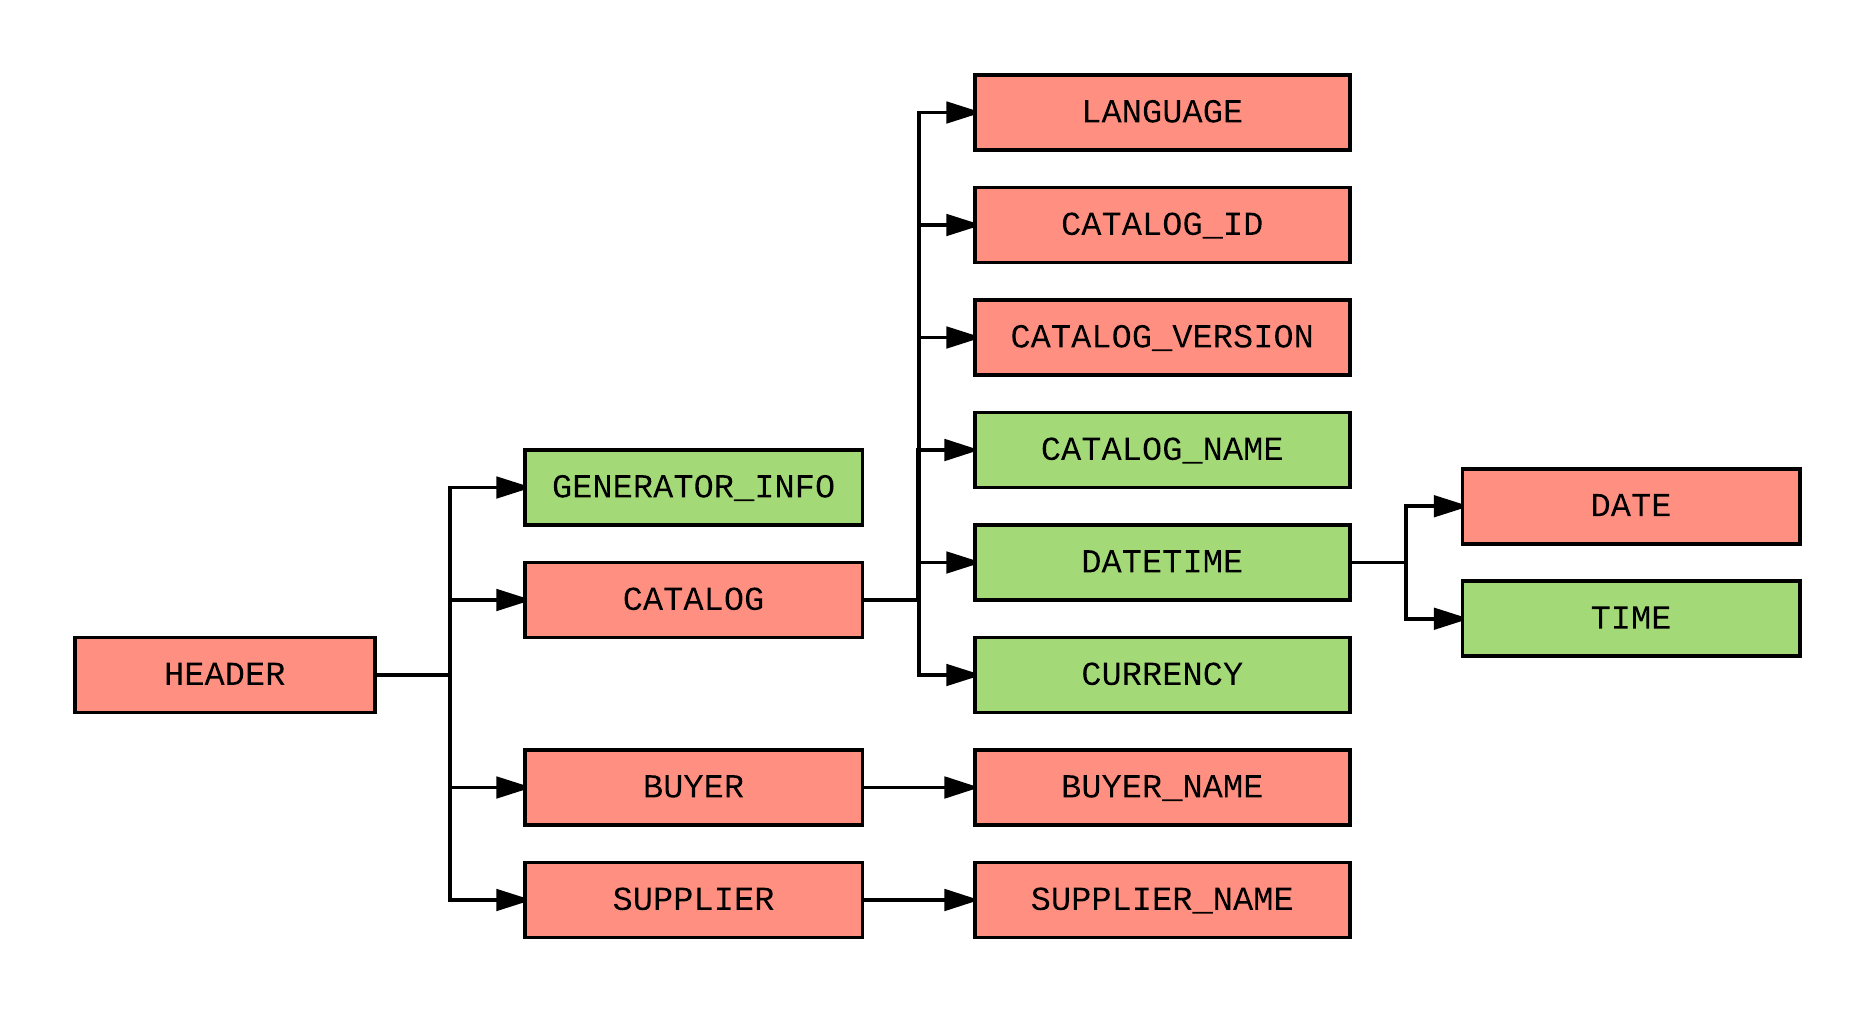
\includegraphics[width=1\linewidth]{img/BMECat_Header}
		\captionof{figure}[Headerstruktur]{Headerstruktur}
		\label{fig:header}
		\vspace{1em}
	\end{minipage}
	
	
	
	\textbf{\underline{Die Transaktion T\_NEW\_CATALOG}}
	
	Diese Transaktion wird verwandt, um einen Produktkatalog neu zu übertragen. Das empfangende System reagiert dabei je nach übertragener \texttt{CATALOG\_ID}, \texttt{CATALOG\_VERSION}
	und \texttt{LANGUAGE} unterschiedlich. Dieser Zusammenhang wir später noch erläutert.
	
	
	\begin{minipage}{\linewidth}
		\vspace{1em}
		\centering
		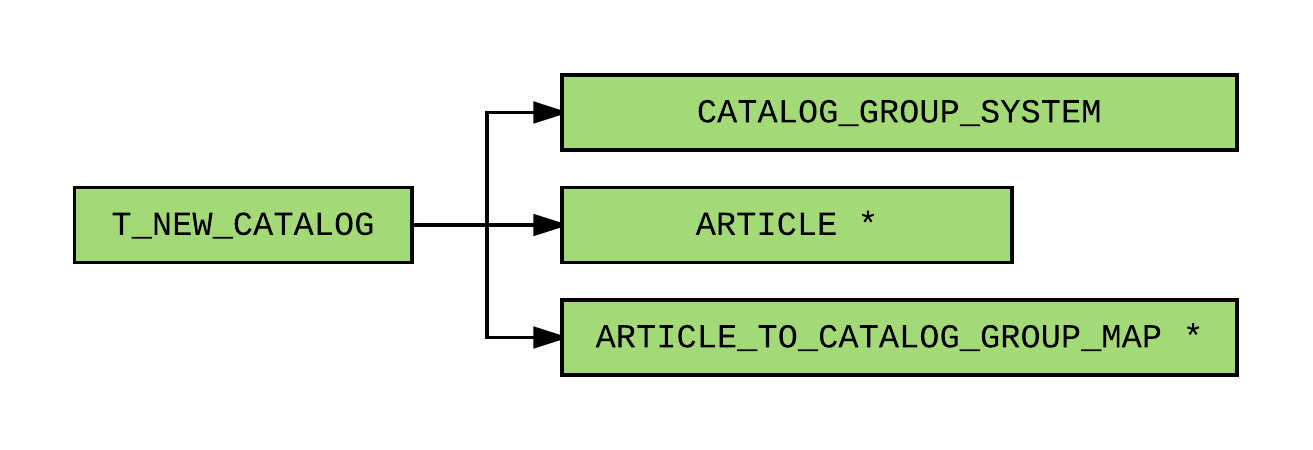
\includegraphics[width=0.8\linewidth]{img/newCatalog}
		\captionof{figure}[T\_NEW\_CATALOG]{T\_NEW\_CATALOG}
		\label{fig:header}
		\vspace{1em}
	\end{minipage}
	
	\textbf{\underline{Die Transaktion T\_UPDATE\_PRODUCTS}}\\
	
	Bei dieser Transaktion werden Artikeldaten übertragen und gegebenenfalls einer Kataloggruppe zugeordnet.Je nach Kennung des Artikels (s.u.)  werden die übertragenen
	Artikel im Zielsystem entweder hinzugefügt, gelöscht oder die Artikeldaten werden komplett ersetzt.
	Der Artikel wird immer komplett ausgetauscht, eine Änderung von einzelnen Datenfeldern innerhalb eines Artikels ist nicht möglich.
	Wie der Grafik entnommen werden kann ist bei dieser Transaktion nur die Übertragung von Produktdaten und die Zuordnung von Produkten zu Kataloggruppen möglich. \footnote{vgl. BMECat V 1.2 Spezifikation, Seite 52}
	
	\begin{minipage}{\linewidth}
		\vspace{1em}
		\centering
		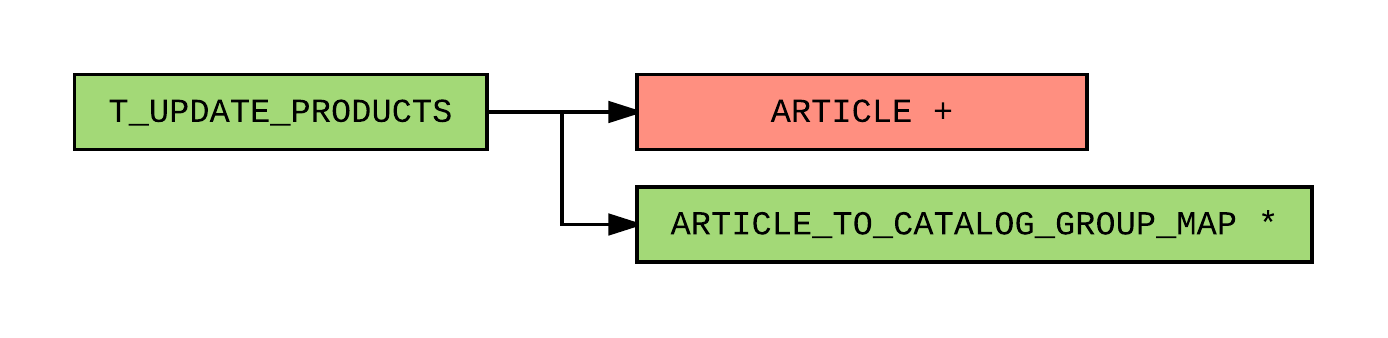
\includegraphics[width=0.8\linewidth]{img/updateProducts}
		\captionof{figure}[T\_UPDATE\_PRODUCTS]{T\_UPDATE\_PRODUCTS}
		\label{fig:header}
		\vspace{1em}
	\end{minipage}
	
	Das Element \texttt{T\_UPDATE\_PRODUCTS} verfügt zusätzlich über das Attribut \texttt{prev\_version}, welches die Anzahl der vorausgegangenen Updates bzw. die Nummer des übertragenen Updates enthält. Der Wer dieses Attributes wird nach jedem Katalogupdate um 1 erhöht.
	
	\begin{lstlisting}
	<T_UPDATE_PRODUCTS prev_version="91">...</T_UPDATE_PRODUCTS>
	\end{lstlisting}
	
	
	
	\textbf{\underline{Die Elemente CATALOG\_GROUP\_SYSTEM und CATALOG\_STRUCTURE}}\\
	
	Im Element \texttt{CATALOG\_GROUP\_SYSTEM} werden die \texttt{GROUP\_SYSTEM\_ID} und der \texttt{GROUP\_SYSTEM\_NAME} bekannt gemacht sowie die Katalogstruktur  \texttt{CATALOG\_STRUCTURE}   beschrieben. Dabei gibt es genau ein Wurzelelement, sowie beliebig viele Knoten und Blätter. Jedes Element hat dabei eine als \texttt{GROUP\_ID} bezeichnete ID und wird über \texttt{PARENT\_ID} die  dem jeweiligen Elternelement zugeordnet. Die Zuordnung der Artikel zu den Artikelgruppen erfolgt mit dem Element \texttt{ARTICLE\_TO\_CATALOG\_GROUP\_MAP} das weiter unten beschrieben wird.
	
	\begin{minipage}{\linewidth}
		\vspace{1em}
		\centering
		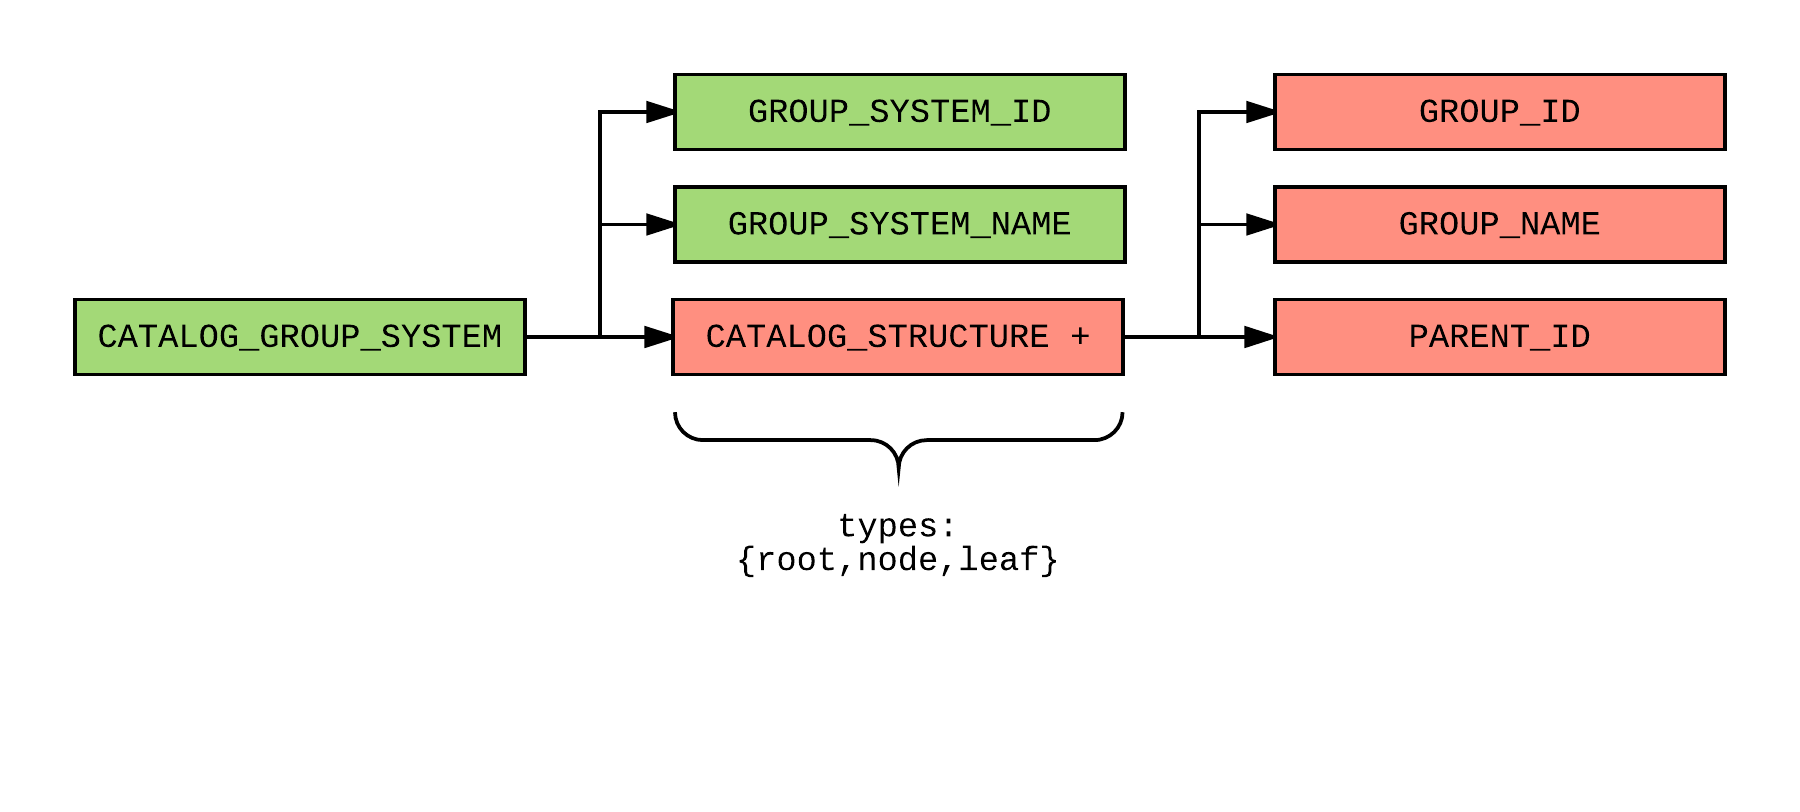
\includegraphics[width=0.6\linewidth]{img/catalogGroupSystem}
		\captionof{figure}[CATALOG\_GROUP\_SYSTEM und CATALOG\_STRUCTURE]{CATALOG\_GROUP\_SYSTEM und CATALOG\_STRUCTURE}
		\label{fig:header}
		\vspace{1em}
	\end{minipage} 
	
	\textbf{\underline{Das Element ARTICLE}}\\
	Das Artikelelement schließlich enthält Informationen über einen Artikel, wie Überschrift, Beschreibung, Bilder, Preisinformationen, eine \textbf{eindeutige} Artikelnummer usw. Die Artikelnummer wird über das Element \texttt{SUPPLIER\_AID} bekanntgegeben, handelt es sich um einen Variantenartikel, so bildet sich die Artikelnummer aus der \texttt{SUPPLIER\_AID} und der \texttt{SUPPLIER\_AID\_SUPPLEMENT}. Dies ist hier jedoch nicht umgesetzt. Die als \textit{eCl@ass} und \textit{Zolltarifnummer} zusammengefassten \texttt{ARTICLE\_FEATURES} werden explizit von Mercateo verlangt.
	
	\begin{minipage}{\linewidth}
		\vspace{1em}
		\centering
		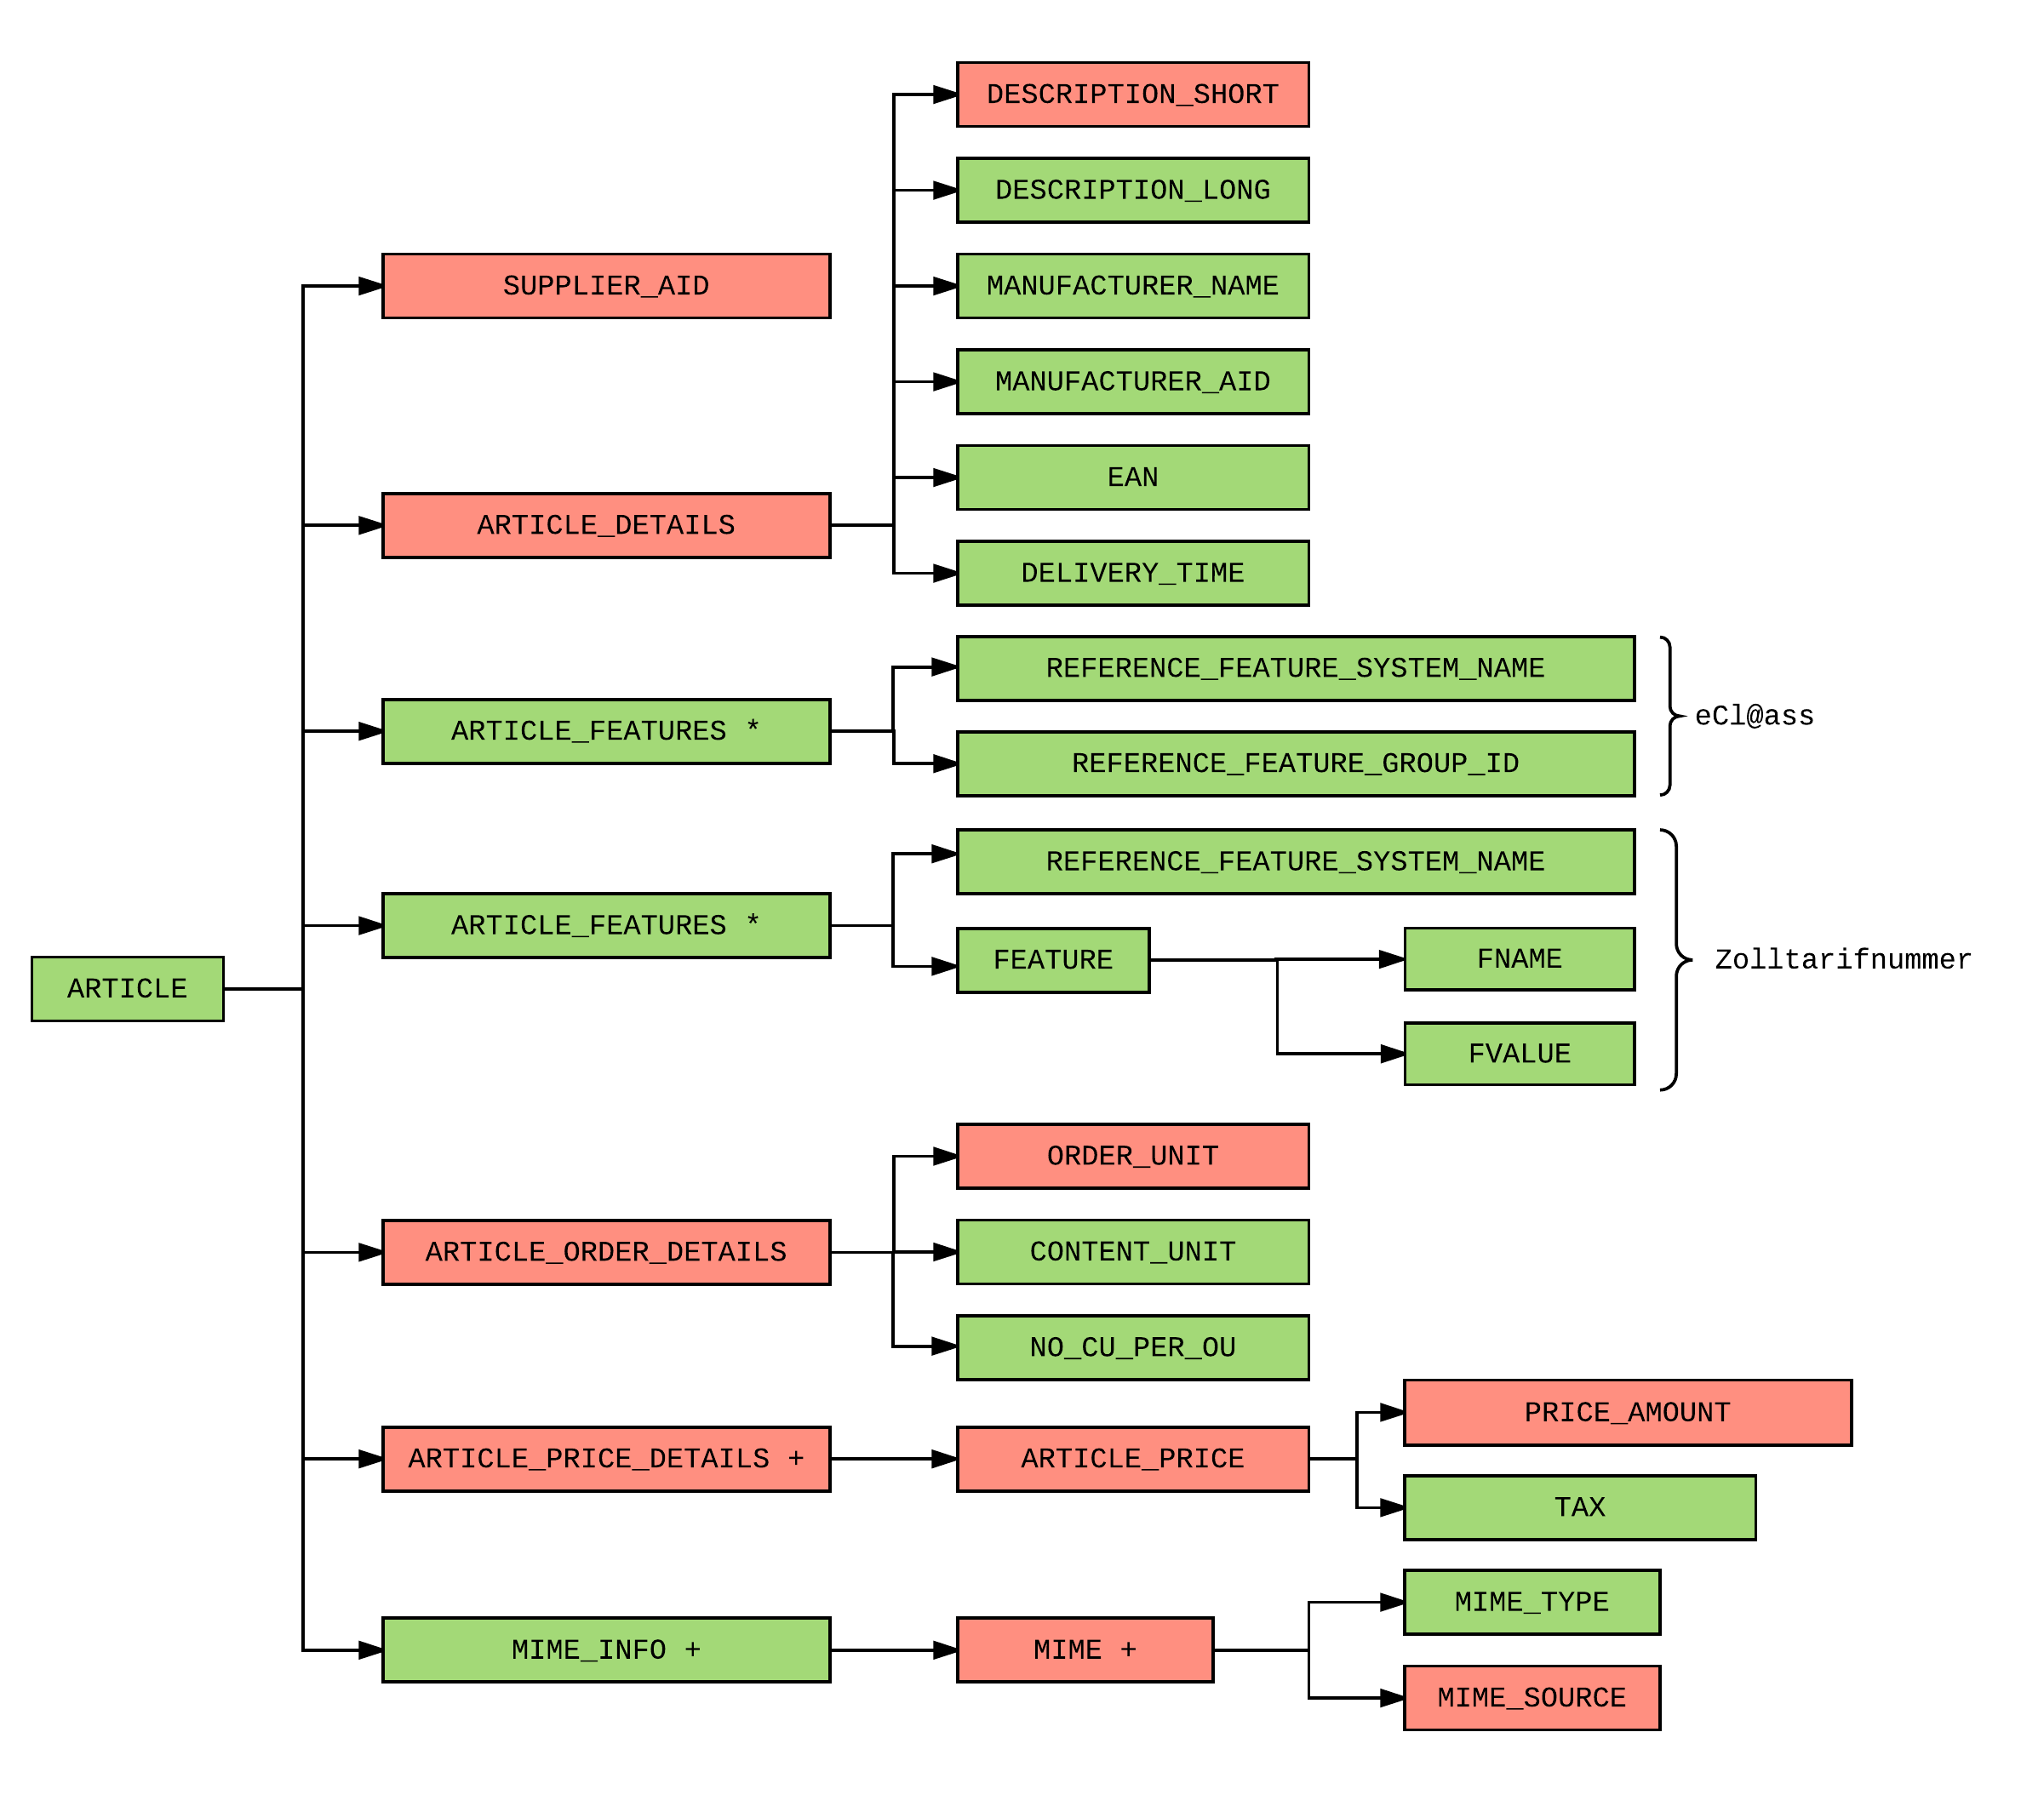
\includegraphics[width=1\linewidth]{img/Article}
		\captionof{figure}[Article]{Article}
		\label{fig:header}
		\vspace{1em}
	\end{minipage}
	
	Das Element \texttt{ARTICLE} verfügt über das Attribut \texttt{mode}, welches Informationen darüber enthält, ob es sich um die Anlage eines neuen Artikel, ein Update der Artikelinformationen oder die Löschung eines Artikels handelt.
	
	\begin{lstlisting}
	<ARTICLE mode="new">...</ARTICLE>
	<ARTICLE mode="update">...</ARTICLE>
	<ARTICLE mode="delete">...</ARTICLE>
	\end{lstlisting}
	
	
	
	\textbf{\underline{Das Element ARTICLE\_TO\_CATALOG\_GROUP\_MAP}}\\
	
	Um Produkte ihren Kategorien zuordnen zu können wird das Element \texttt{ARTICLE\_TO\_CATALOGGROUP\_MAP} verwandt. Es erfolgt hier eine Verknüfung aus der eindeutigen Artikelnummer und der \texttt{GROUP\_ID} welcher der Artikel zugeordnet werden soll. Eine Mehrfachzuordnung ist möglich, d.h. ein Artikel kann in unterschiedliche Kategorien "eingehängt" werden.
	
	\begin{minipage}{\linewidth}
		\vspace{1em}
		\centering
		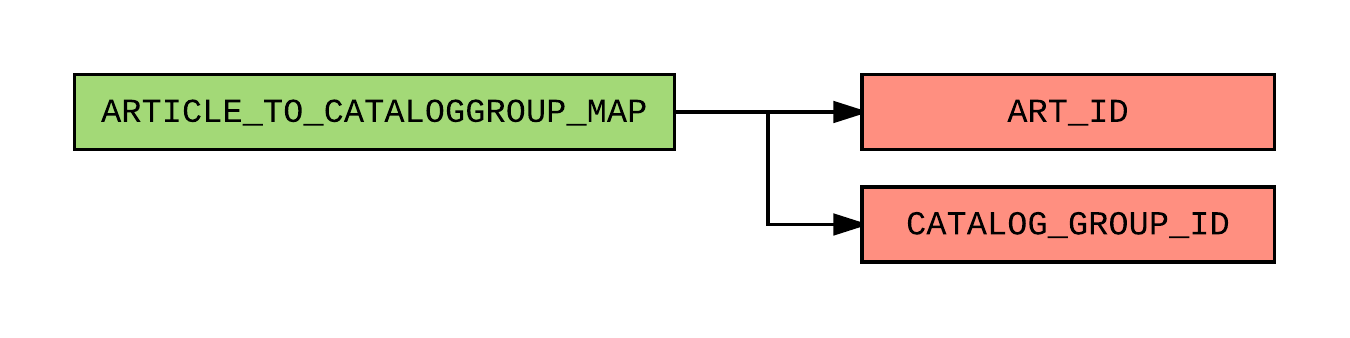
\includegraphics[width=0.7\linewidth]{img/articleGroupMap}
		\captionof{figure}[ArticleGroupMap]{ARTICLE\_TO\_CATALOG\_GROUP\_MAP}
		\label{fig:header}
		\vspace{1em}
	\end{minipage}
	
	Im Kontext der Transaktion \texttt{T\_UPDATE\_PRODUCTS} verfügt das Element zusätzlich über das Attribut \texttt{mode}, mit welchem angegeben wird, ob es sich um eine Neuzuweisung zu einer Kategorie handelt oder der Artikel aus einer Kategorie entfernt werden soll.
	
	\begin{lstlisting}
	<ARTICLE_TO_CATALOGGROUP_MAP mode="new">...</<ARTICLE_TO_CATALOGGROUP_MAP>
	<ARTICLE_TO_CATALOGGROUP_MAP mode="delete">...</<ARTICLE_TO_CATALOGGROUP_MAP>
	\end{lstlisting}
	
	
	\textbf{\underline{Zusammenspiel verschiedener Transaktionen}}\\
	
	Die folgende Grafik zeigt, wie das empfangende System bei der Transaktion \texttt{T\_NEW\_CATALOG} je nach übergebener \texttt{CATALOG\_ID}, \texttt{CATALOG\_VERSION} und \texttt{LANGUAGE} reagiert.
	
	\begin{minipage}{\linewidth}
		\vspace{1em}
		\centering
		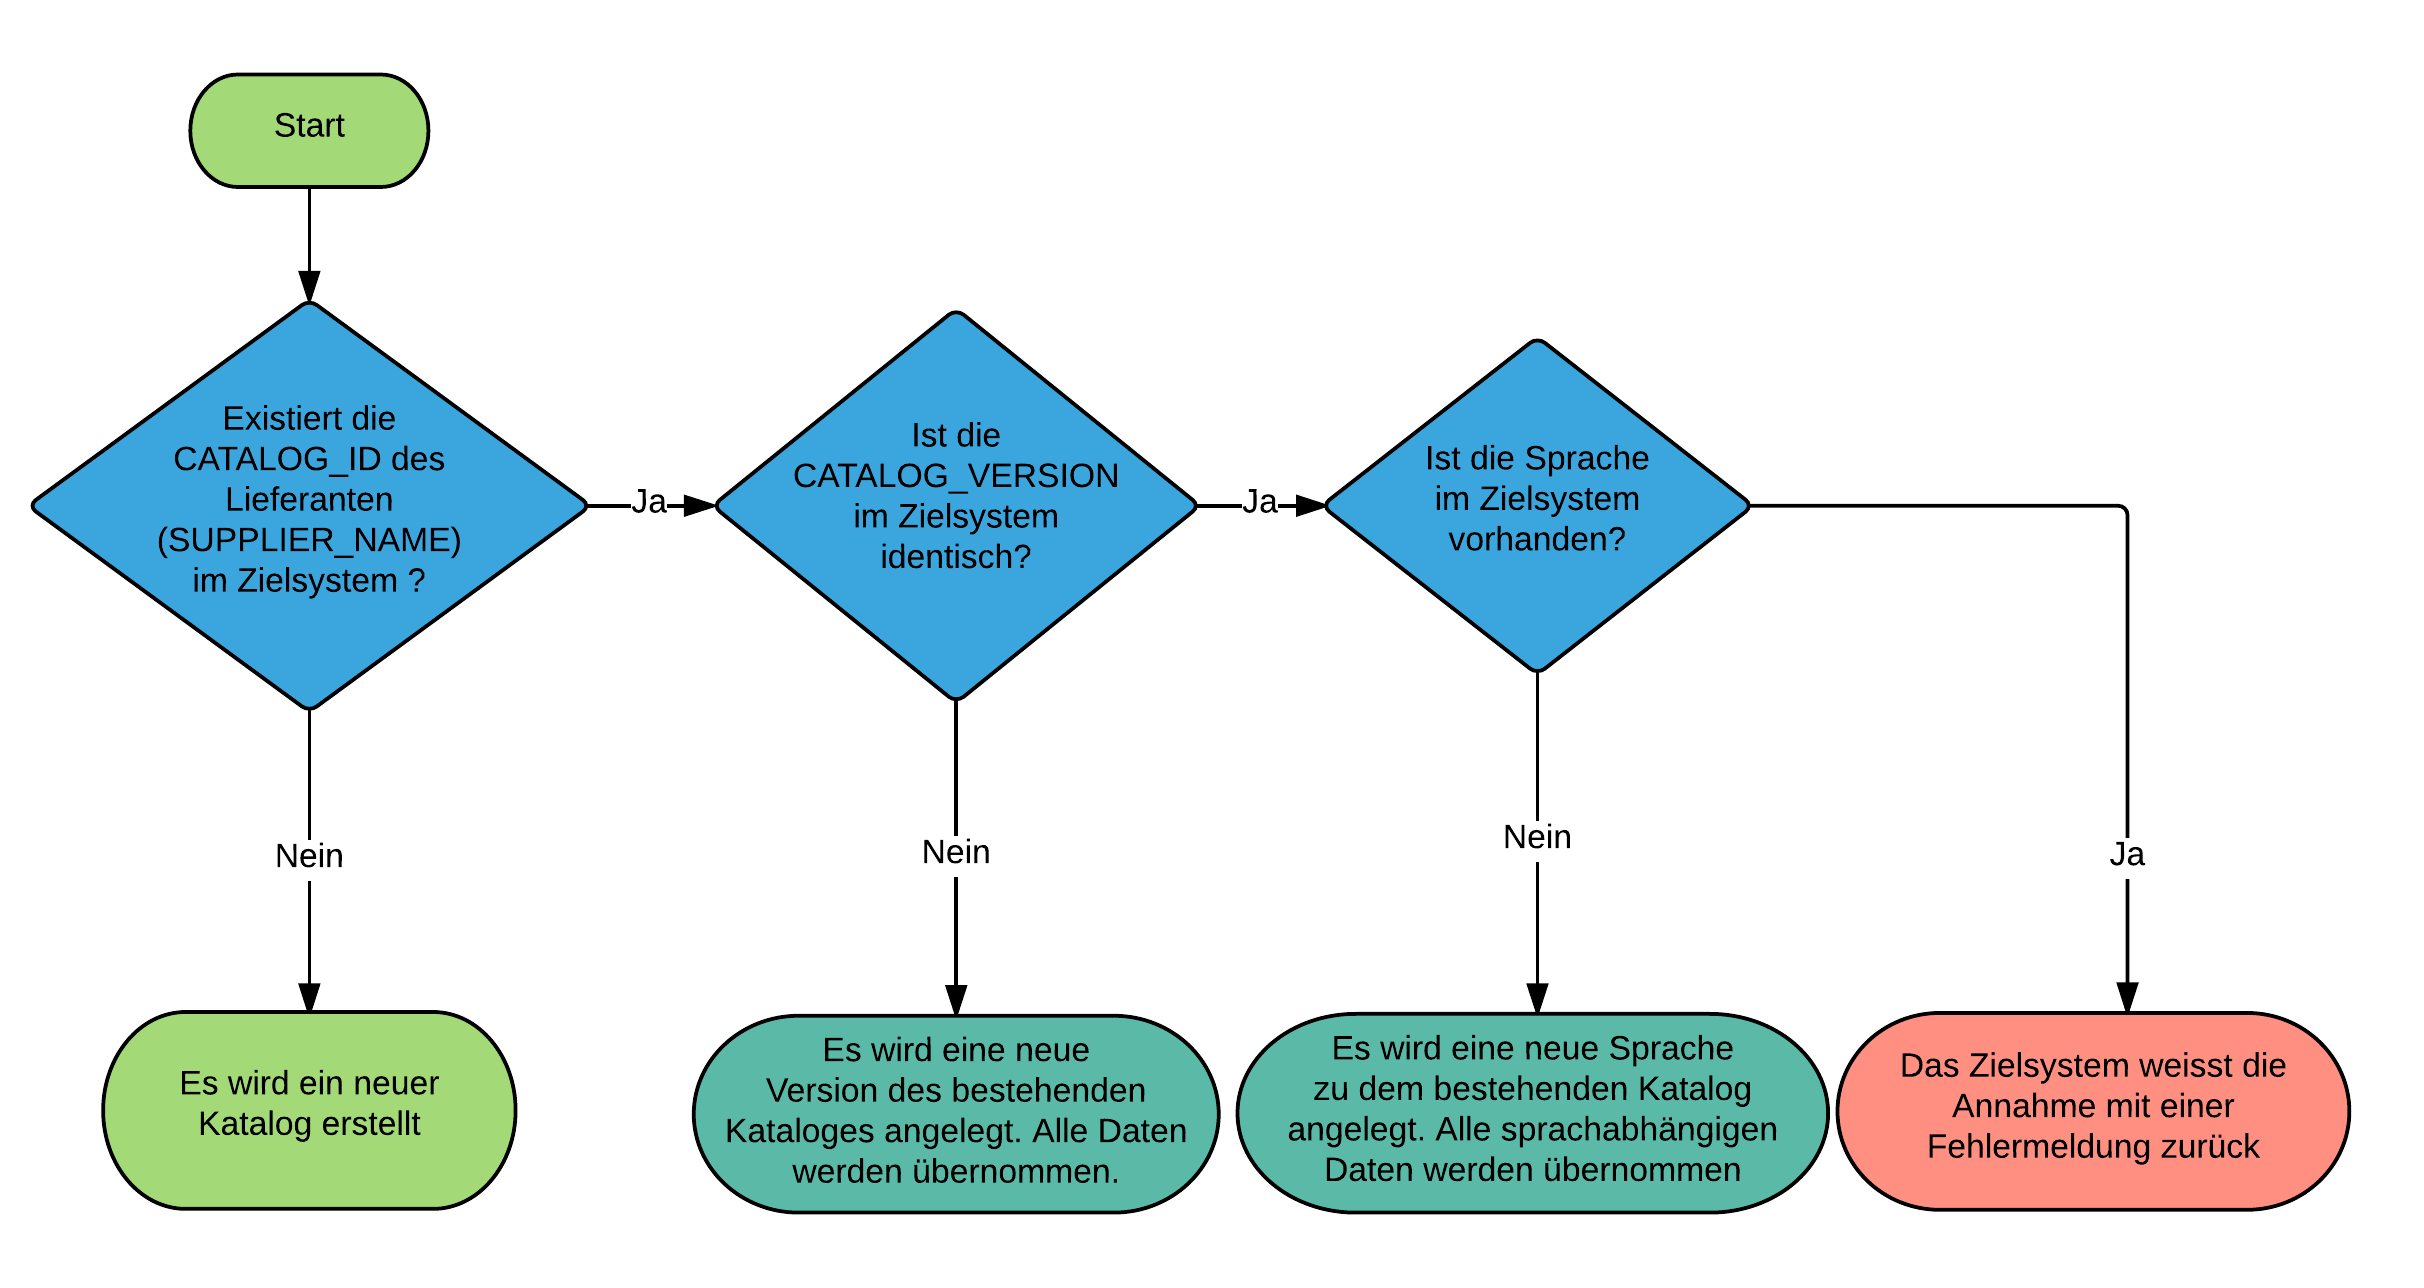
\includegraphics[width=0.65\linewidth]{img/newCatalogLogik}
		\captionof{figure}[New Catalog Logik]{Flowchart T\_NEW\_CATALOG}
		\label{fig:header}
		\vspace{1em}
	\end{minipage}
	
	Kommt die Transaktion \texttt{T\_UPDATE\_PRODUCTS} zur Anwendung, gilt es folgendes zu beachten:\footnote{vgl. hierzu: BMECat V 1.2 Spezifikation, Seite 52} 
	\begin{itemize}
		\item Die übertragene \texttt{CATALOG\_ID} des jeweiligen Lieferanten und die dazugehörige\\ \texttt{CATALOG\_VERSION} müssen im Zielsystem bereits vorhanden sein.
		\item Das Attribut \texttt{prev\_version} muss bei der ersten anderen Transaktionsart nach\\ \texttt{T\_NEW\_CATALOG}, (\texttt{T\_UPDATE\_PRODUCTS},\texttt{T\_UPDATE\_PRICES}) auf '0' gesetzt werden.
		\item Danach wird es bei jeder solchen Transaktion um '1' erhöht.
	\end{itemize}
	
	
	---- Übersicht, tabellarisch oder nicht über die wichtigsten Felder und ihre Einschränkungen, vor allem die von Mercateo ----
	
	\subsection{Das Cake-PHP Framework}
	
	Cake PHP ist ein Webframework, das dem MVC (Model-View-Controller) Schema folgt und dabei die Softwaredesignparadigmen DRY (Don't repeat yourself) und 'Convention over configuration' umsetzt. 
	
	\subsubsection{Convention over Configuration in CakePHP}
	
	%Hier noch eine Erklärung zu COC von den Big Five einfügen
	In CakePHP wird das Softwaredesign-Paradigma der 'Konvention vor Konfiguration' konsequent umgesetzt.\newline 
	
	 Die Klassennamen von \textbf{Controllern} sind im Plural verfasst, 'CamelCased' und enden auf \textit{Controller}. \texttt{UsersController} und \texttt{ArticleCategoriesController} sind Beispiele dafür. Eine öffentliche Methode eines solchen Controllers kann über einen Webbrowser aufgerufen werden. Per Konvention werden URLs klein geschrieben und mit Bindestrich verbunden.
	\url{http://samplesite.com/article-categorie/view} ruft demnach die öffentliche \texttt{view()} Methode des ArticleCategoriesControllers auf.\\
	\newline
	Die Namen von \textbf{Model} Klassen sind 'CamelCased' und im Plural. Der Name der zum Model gehörenden Tabelle ist im Plural verfasst und mit einem Unterstrich verbunden.\\
	\texttt{article\_categories} ist die dem Model \texttt{ArticleCategories} zugrundeliegende Tabelle. Um einen Fremdschlüssel auf eine Tabelle zu vergeben genügt es das Suffix \texttt{\_id} an den kleingeschriebenen Namen dieser Tabelle anzuhängen. Wenn Users eine hasMany Beziehung zu Articles hat, kann mit dem Fremdschlüssel \texttt{user\_id} in der \texttt{articles}-Tabelle auf den entsprechenden Eintrag in der \texttt{users}-Tabelle verwiesen werden. \newline
	
	Die Template Datei einer \textbf{View} ist nach der entsprechenden Methode im Controller benannt die sie darstellen soll. Die \texttt{view()} Methode der \texttt{ArticlesController} Klasse würde demnach unter \texttt{src/Template/Articles/view.ctp} nach einem View-Template suchen\footnote{vgl. hierzu: \url{http://book.cakephp.org/3.0/en/intro/conventions.html}}.
	
	\subsubsection{Model}
	
	Das Backend einer CakePHP Anwendung wird von einer SQL Datenbank gebildet. Das Model repräsentiert die Daten einer Anwendung und enthält die Geschäftslogik zur Datenmanipulation. Nach der CakePHP Konvention wird die Datenbankverbindung einmal in der \texttt{config/app.php} konfiguriert. Die Model-Klasse stellt dabei Methoden zur Verfügung, über die es möglich ist, den Zustand der Daten abzufragen, die Daten zu filtern und zu verändern. Die CRUD-Funktionalität (CREATE-READ-UPDATE-DELETE) ist so direkt im Model integriert.\footnote{vgl. hierzu: Webentwicklung mit CakePHP, 2. Auflage, O'Reilly, Seite 7}. 
	Die Beziehungen einzelner Models zueinander werden über \textit{Associations} hergestellt. Die vier Assoziationstypen in CakePHP sind:\\

	
		\begin{tabularx}{\textwidth}{p{1cm} X X p{8cm}}
		\cline{2-4}
		\rowcolor[HTML]{EFEFEF} 
		 Nr. & Beziehung & Typ & Beispiel \\ \cline{1-4} \addlinespace
		1. & one to one & hasOne & Ein Museum hat eine Adresse. \\
		2. & one to many & hasMany & In einem Museum hängen mehrere Kunstwerke. \\
		3. & many to one & belongsTo & Mehrere Bilder gehören zu einem Museum. \\  
		4. & many to many & belongsToMany & Ein Student hat mehrere Professoren. Ein Professor hat mehrere Hörer. \\ \addlinespace \cline{1-4}     
		\end{tabularx}
	\\
	
	
	Es ist möglich ein \textit{Model} um ein oder mehrere \textit{Behavior} zu erweitern. Dabei handelt es sich um Klassen, in denen, ähnlich einem Trait, Funktionen zur Erweiterung des Models gekapselt sind. Ein Beispiel hierfür ist das Tree-Behavior, das es ermöglicht hierarchische Datenstrukturen in der Datenbank zu pflegen. Anwendung hierfür kann z.B. die Abbildung einer Kategoriestruktur sein \footnote{vgl. hierzu: \url{http://book.cakephp.org/3.0/en/orm/behaviors/tree.html}}.
	
	Mit Hilfe von im Model definierten Validatoren können zu speichernde Daten auf Vollständigkeit und Konsistenz geprüft werden. 
	
	 Später bei der Beschreibung des Codes auf eigenen Validator verweisen. (MercateoAccountsTable::validateCatalogVersionFormat)
	\lstset{language=PHP}
	\begin{lstlisting}

	$validator
     	->requirePresence('catalog_name', 'create')
     	->notEmpty('catalog_name')
     	->add('catalog_name', [
	         'maxLength' => [
	             'rule' => ['maxLength', 100],
	             'message' => 'maxLength = 100.'
	         ]
     ]);
	
	\end{lstlisting}
	
	\subsubsection{View}
	
	Die View ist für die Darstellung der Daten in der Anwendung zuständig. Eine View ist in CakePHP immer auf ein bestimmtes Model bezogen und wird nicht für die Darstellung anderer Daten verwendet\footnote{vgl. hierzu: Webentwicklung mit CakePHP, 2. Auflage, O'Reilly, Seite 7}. CakePHP View Template Dateien Enden auf '.ctp' und bedienen sich der alternativen PHP Syntax für Kontrollstrukturen und Ausgabe. 
	In einer View kann direkt auf Variablen zugegriffen werden die in der entsprechenden Controller Methode gesetzt wurden:\\ 
   \lstset{language=PHP} 
	\begin{lstlisting}
	$this->set('articleCategories',  $articleCategories);
	\end{lstlisting}
	  Die Codebeispiele zeigen, wie die Variable \texttt{\$articleCategories} im Controller für die View freigegeben wird und dort z.B. mit einer foreach-Schleife durchlaufen werden kann um ihren Inhalt auszugeben. 
		\lstset{language=PHP}
		\begin{lstlisting}[caption={Alternative PHP Syntax}] 	
		<ul>
	   	<?php foreach ($todo as $item): ?>
		  <li><?= $item ?></li>
		<?php endforeach; ?>
		</ul>
		\end{lstlisting}
	 Eine View ist dabei nicht auf das Anzeigen von HTML Inhalten beschränkt, sondern kann auch dazu verwandt werden XML- oder JSON- Repräsentationen der angefragten Daten zurückzuliefern.
	\subsubsection{Controller}
	Der Controller regelt den Ablauf der Benutzerinteraktion.
	Er ist dafür zuständig, dass das richtige Model aufgerufen und die entsprechende Antwort oder View erzeugt wird. Er dient dabei als eine Art Vermittler zwischen dem Model und der View. Normalerweise ist in CakePHP ein Controller für ein Model verantwortlich, es ist dennoch möglich, oft auch nötig, dass ein Controller mit mehreren Models arbeitet.
	
	Der Controller enthält eine Reihe von  Methoden die HTTP Anfragen verarbeiten. Diese Methoden werden in CakePHP \textit{actions} genannt. Per Definition ist jede öffenliche Methode in einem Controller eine \textit{action} und über eine URL der Form \url{http://samplesite.com/article-categorie/view} erreichbar.
	Eine \textit{action} ist für die Verarbeitung der Anfrage und das zurückliefern einer Antwort zuständig. Im normalfall wird dabei eine View erzeugt, es können aber auch (wie im Abschnitt Model erläutert) auch XML oder JSON Daten zurückgeliefert werden.\footnote{vgl. hierzu: \url{http://book.cakephp.org/3.0/en/controllers.html}}
	
	\subsubsection{Component}
	Komponenten (Components) sind in sich geschlossene Bereiche innerhalb einer Applikation, die eine bestimmte Funktionalität kapseln und über die Grenzen eines Controllers hinaus verfügbar machen. Sollen bestimmte logische Prozesse in verschiedenen Teilen einer Anwendung zur Verfügung stehen - insbesondere in unterschiedlichen Controllern- so ist es sinnvoll diese in eine Komponente auszulagern.\footnote{vgl hierzu: CakeBuch Webentwcik, Seite 223}
	Die Möglichkeit mit Komponenten zu arbeiten setzt das DRY Paradigma konsequent um.
	
	\subsubsection{Shell}	
	CakePHP bietet die Möglichkeit Konsolenanwendungen zu schreiben. Dies ist nützlich für Anwendungen die per Cronjob ausgeführt werden sollen oder für solche die nicht aus einem Browser erreicht werden müssen bzw. sollen. \texttt{vgl. hierzu \url{http://book.cakephp.org/3.0/en/console-and-shells.html}}
	Eine der wichtigsten Funktionalität der Cake Shell ist das 'Backen' (Baking). Gemeint ist damit die automatische Generierung von Code. Der Befehl \texttt{bin/cake bake} erstellt, je nach gewählter Option, ganze MVC Grundgerüste, Controller- oder Model- Klassen, Plugin Verzeichnisstrukturen oder Shell-Klassen. Einzelne Funktionalitäten einer Shell Klasse können in Tasks ausgelagert werden.  
	
	\subsubsection{Einschätzung}
	
	
	
	\section{Analyse der Aufgabe und der Anforderungen}
	
	\subsection{Bewertung von theoretischen Ansätzen, Konzepten, Methoden, Verfahren}
		Im folgenden sollen die verwendeten Technologien bewertet werden. 
		Wie gut sind sie jeweils für den Einsatzzweck geeignet?
		Bewertungskriterien sind: 
		
		
	\subsubsection{CakePHP-Framework}
	
	
	
	\subsubsection{SQL Datenbank}
	
	
	\subsubsection{BMECat Format}
	
	Allgemeine Vorteile die sich aus dem XML-Format ergeben sind die gleichzeitige Mensch- und Maschinenlesbarkeit sowie die Möglichkeit das Dokument gegen ein XML-Schema testen zu können. So kann schon direkt nach der Erzeugung des BMECat Dokumentes überprüft werden, ob die geschriebenen Elemente vom richtigen Datentyp sind und das Dokument der in der XSD Datei festgelegten Struktur folgt. Weitere Vorteile speziell des BMECat Standards sind\footnote{vgl. hierzu: \url{http://wiki.prozeus.de/index.php/BMEcat}}:
	
	\begin{itemize}[noitemsep]
	\item konfigurierbare Produkte sind abbildbar
	\item mehrsprachige Kataloge sind in einem Katalogdokument abbildbar
	\item Übermittlung multimedialer Datenelemente ist möglich (z.B. Produktvideos)	
	\item gilt zumindest in Deutschland als etabliertes Katalogaustauschformat	
	\end{itemize}
	
	
	
	\subsubsection{Datenübertragung zu Mercateo}
	
	Die Übertragung der Katalogdatei zum Mercateo-Server geschieht über FTP. Neue Dateien werden alle 30 Minuten vom Mercateo-System verarbeitet.\\
	\textbf{Vorteile:}
 	\begin{itemize}[noitemsep]
   	\item einfach anzuwenden.
   	\item Eine korrekte Datenübertragung ist durch die Fehlerbehandlung von TCP gewährleistet.
   	\end{itemize}
	\textbf{Nachteile:}
   	\begin{itemize}[noitemsep]
   	\item Datenübertragung nicht nach außen abgesichert.
   	\item Übertragene Daten können mitgelesen und manipuliert werden.
   	\item Benutzerkennung und Passwort können abgefangen werden
   	\end{itemize}
   	\textbf{Fazit:}\\
	Nicht optimal, vor allem aus Sicherheitsgründen. Zudem Fehleranfällig, wenn die Ordnerstruktur- und Dateinamenskonventionen von Mercateo nicht eingehalten werden \footnote{vgl. hierzu \url{http://www.mercateo.com/support/verkaufen/katalog-allgemeine-informationen/datenuebertragung-per-ftp/}}.

		
		
	\subsection{Funktionale und nichtfunktionale Anforderungen}	
			- 
	
	\subsection{Informelle Aufgabenbeschreibung}
	Ziel der Arbeit ist es die von der Software iTool aus verwaltbaren, in verschiedenen Tabellen einer SQL-Datenbank gehaltenen Produkt-, Katalog- Kategorie- und Herstellerdaten in ein von Mercateo verarbeitbares Format (dem BMECat) zu bringen. Dabei gilt es, den Anforderderungen der Spezifikationen sowohl das BMECat, als auch der besonderen Anforderungen seitens Mercateo zu genügen.
	Es soll möglich sein, die erwähnten Daten aus dem UI des iTool heraus nach dem CRUD-Prinzip zu bearbeiten. 
	Die eigentliche Erstellung der unterschiedlichen Kataloge (neuer Katalog bzw. Produktupdatekatalog) erfolgt dabei (automatisiert) über die CakePHP Shell. Kataloge können dabei für unterschiedliche Verkäufer erstellt werden.
	Zudem soll es Meracteo ermöglicht werden Bestandsdaten zu einer bestimmten Artikelnummer über ein Webinterface abzurufen.
	
	\subsection{Zielstellung}
	
	Folgende Funktionalitäten sollen implementiert werden:
	
	\begin{itemize}[noitemsep]
	\item Die in iTool hinterlegten Produkt- bzw. Herstellerdaten sollen in ein gültiges und vollständiges BMECat Dokument entsprechend der Mercateo Anfoderungen überführt werden. Dabei ist insbesondere auf die Unterschiede und Besonderheiten der notwendigen beiden Transaktionsarten \texttt{T\_NEW\_CATALOG} - also die Erstellung eines neuen Kataloges - und \texttt{T\_UPDATE\_PRODUCTS} - also der Änderungen von Produktdaten, sowie dem löschen und neu erstellen von Produkten - zu achten .
		\begin{itemize}[noitemsep]
		\item Gültig bedeutet in diesem Fall, dass Struktur und Inhalt des Dokuments fehlerfrei gegen die entsprechende XSD Datei laufen, d.h. die Felder müssen in der richtigen Reihenfolge unter Beachtung der Datentypen und Längenbegrenzungen sowie Formatlimitierungen (z.B. keine Sonderzeichen in der SKU (o.ä.)) geschrieben werden.
		\item Vollständig heißt, dass zum einen mindestens jene Felder im BMECat Dokument vorkommen, die die BMECat Spezifikation verlangt.Zusätzlich müssen jene Felder vorkommen, die die Mercateo Spezifikation erfordert und zwar unter zusätzlicher Beachtung der Limitierungen bzw. Besonderheiten jener Spezifikation. 	
		\end{itemize}
		
	\item Die Produktkategoriestruktur des iTool soll in das Kataloggruppensystem des BMECat überführt werden.
	\item die Implementierung der Katalogerstellungslogik erfolgt in einer Cake Shell. Liegt noch kein Katalog vor, wird ein neuer Katalog erstellt; ein Updatekatalog wird erstellt, wenn es Änderungen bei den Produktdaten gab. 
	\item Kataloge können für unterschiedliche Verkäufer erstellt werden.
	\item Die Produkt und Katalogdaten können über die Benutzeroberfläche des iTool eingesehen bzw. verändert werden. 
	\item Es soll Mercateo ermöglicht werden Bestandsdaten zu den im Katalog vermerkten Produkten über ein Webinterface abzurufen.
	\item Bei der Katalogerstellung ist darauf zu achten, dass es zu keinen Arbeitsspeicherüberläufen kommen kann.
	\end{itemize}
	
	\section{Entwurf}	
	
	
	
	\subsection{Katalogerstellung}
	
	Die Erstellung der BMECat Dokumente wird über eine CakePHP Shell realisiert. Das hat den Vorteil, dass diese über einen Cronjob automatisiert werden kann werden kann. Um die Shell im Bedarfsfall leicht erweitern zu können und nicht zu überladen wird die Logik in einen Shell-Task \texttt{prepareCatalog} ausgelagert.Es soll möglich sein beim Aufruf des Tasks die \textit{id} des \texttt{core\_sellers} zu übergeben, dessen Produkte exportiert werden sollen. Die Spezifikation des BMECat verlangt, dass im Katalogdokument bestimmte Informationen zur Katalogversion, dem Katalognamen, der Währung \textit{etc.} aufgeführt werden. Diese Daten werden in der Tabelle \texttt{mercateo\_accounts} gespeichert und können über die GUI des iTool eingesehen, erstellt, gelöscht und geändert werden. 
	
	\subsubsection{Die Tabelle \texttt{mercateo\_accounts}}
	
	Eine Übersicht der in \texttt{mercateo\_accounts} gespeicherten Werte bietet folgende Tabelle, wenn nicht anders angegeben entspricht das BMECat Element der Spaltenbezeichnung (\texttt{catalog\_id} == \textless CATALOG\_ID \textgreater )


	\begin{tabularx}{\textwidth \small}{p{4cm} X p{3cm} }
		\rowcolor[HTML]{EFEFEF} 
		Spalte & Erläuterung & BMECat Element \\ \cline{1-3} \addlinespace[7pt]
		id & Primärschlüssel & \multicolumn{1}{c}{\normalsize$\times$} \\
		core\_seller\_id & Fremdschlüssel auf \texttt{core\_sellers}  & \multicolumn{1}{c}{\normalsize$\times$}  \\ 
		core\_marketplace\_id & Fremdschlüssel auf \texttt{core\_marketplaces} & \multicolumn{1}{c}{\normalsize$\times$} \\ 
		core\_currency\_id & Fremdschlüssel auf \texttt{core\_marketplaces}  & \textless CURRENCY \textgreater \\ 
		supplier\_name & Name des verkaufenden Unternehmens & \multicolumn{1}{c}{\normalsize \checked}   \\
		catalog\_id & Eindeutiger Bezeichner des Produktkataloges & \multicolumn{1}{c}{\normalsize \checked}  \\
		catalog\_version & Eindeutiger Bezeichner des Produktkataloges & \multicolumn{1}{c}{\normalsize \checked} \\
		catalog\_name & Eindeutiger Bezeichner des Produktkataloges & \multicolumn{1}{c}{\normalsize \checked} \\
		group\_system\_id & Eindeutiger Bezeichner des Produktkataloges & \multicolumn{1}{c}{\normalsize \checked}  \\
		group\_system\_name & Eindeutiger Bezeichner des Produktkataloges & \multicolumn{1}{c}{\normalsize \checked}  \\
		group\_system\_description & Eindeutiger Bezeichner des Produktkataloges & \multicolumn{1}{c}{\normalsize \checked} \\
		
		
		
		
		
		created & Timestamp, wann der Eintrag erzeugt wurde & text \\
		modified & Timestamp, wann der Eintrag geändert wurde & text \\\addlinespace[7pt] \cline{1-3} 
		\end{tabularx}%
	
	
	

	
	
	
	
	 
	\subsubsection{Die Tabelle \texttt{mercateo\_products}}

	Im Zentrum der Katalogerstellung steht die Tabelle mercateo\_products. Sie dient als Zwischenspeicher für die in \texttt{core\_products} gespeicherten Daten und gibt Auskunft darüber, ob (und wann) Produkte geändert, gelöscht oder neu hinzugefügt wurden. Dadurch wird sie zum zentralen Element zur Umsetzung der Transaktionen \texttt{T\_NEW\_CATALOG} und \texttt{T\_UPDATE\_PRODUCTS}. 
	
	\begin{tabularx}{\textwidth}{p{4cm} X}
	\rowcolor[HTML]{EFEFEF} 
	Spalte & Erläuterung \\ \cline{1-2} \addlinespace[7pt]
	id & Primärschlüssel \\
	core\_product\_id & Fremdschlüssel auf core\_products Tabelle \\
	core\_categorie\_id & Kategorie ID  \\
	status & Der Status des Eintrages \\
	sku & Die SKU des Artikels \\
	title & Die 'DESCRITION\_SHORT' des Artikels  \\ 
	created & Timestamp, wann der Eintrag erzeugt wurde  \\
	modified & Timestamp, wann der Eintrag geändert wurde  \\\addlinespace[7pt] \cline{1-2} 
	\end{tabularx}%
	
	Die Spalten 'sku','core\_category\_id' \& 'title' sind notwendig einen Artikel in einem BMECat Dokument als \textit{gelöscht} auszeichnen zu können. Die Spalte 'status' akzeptiert vier  \textit{Zustände}: 
	

	\begin{tabularx}{\textwidth}{p{3cm} X}
	\rowcolor[HTML]{EFEFEF} 
	Zustand & Erläuterung \\ \cline{1-2} \addlinespace[7pt]
	\texttt{new} & Produktdaten wurden neu in \texttt{core\_products} angelegt. \\
	\texttt{update} & Produktdaten wurden geändert. \\
	\texttt{delete} & Produktdaten wurde aus \texttt{core\_products} gelöscht. \\
	\texttt{active} & Produktdaten wurden in das aktuelle BMECat Dokument übernommen. \\
	   \addlinespace[7pt] \cline{1-2} 
	\end{tabularx}%
		
	Diese Zustände sind die Werte die das Attribut \texttt{mode} des BMECat Elements \texttt{ARTICLE} annehmen kann. Gleichzeitig geben sie an dieser Stelle Auskunft darüber ob ein in \texttt{core\_products} gespeicherter Datensatz neu ist bzw. gelöscht oder verändert wurde. Jene Datensätze die in das aktuelle BMECat Dokument geschrieben wurden, werden mit 'active' markiert.
	
	\subsubsection{Allgemeiner Programmablauf}
	
	
	
	\subsubsection{Katalogerstellungslogik bei der Transaktion \texttt{T\_NEW\_CATALOG}}
	
	Mit dem ersten Programmaufruf wird die \texttt{mercateo\_products} Tabelle mit den entsprechenden Werten aus \texttt{core\_products} initialisiert. Allen Einträgen wird dabei zunächst der Status \texttt{new} zugewiesen. Zugleich werden Datum \& Uhrzeit der Initialisierung in die Tabelle \texttt{core\_configurations} geschrieben. Diese Tabelle ist bereits in iTool angelegt und dient als zentraler Ort um Konfigurationsdaten abzulegen. Anschließend wird eine BMECat Datei mit der Transaktion \texttt{T\_NEW\_CATALOG} erstellt, die Katalogversion in \texttt{core\_configurations} geschrieben und der Status aller Einträge in \texttt{mercateo\_products} auf \texttt{active} gesetzt. 
	
	\begin{minipage}{\linewidth}
		\vspace{1em}
		\centering
		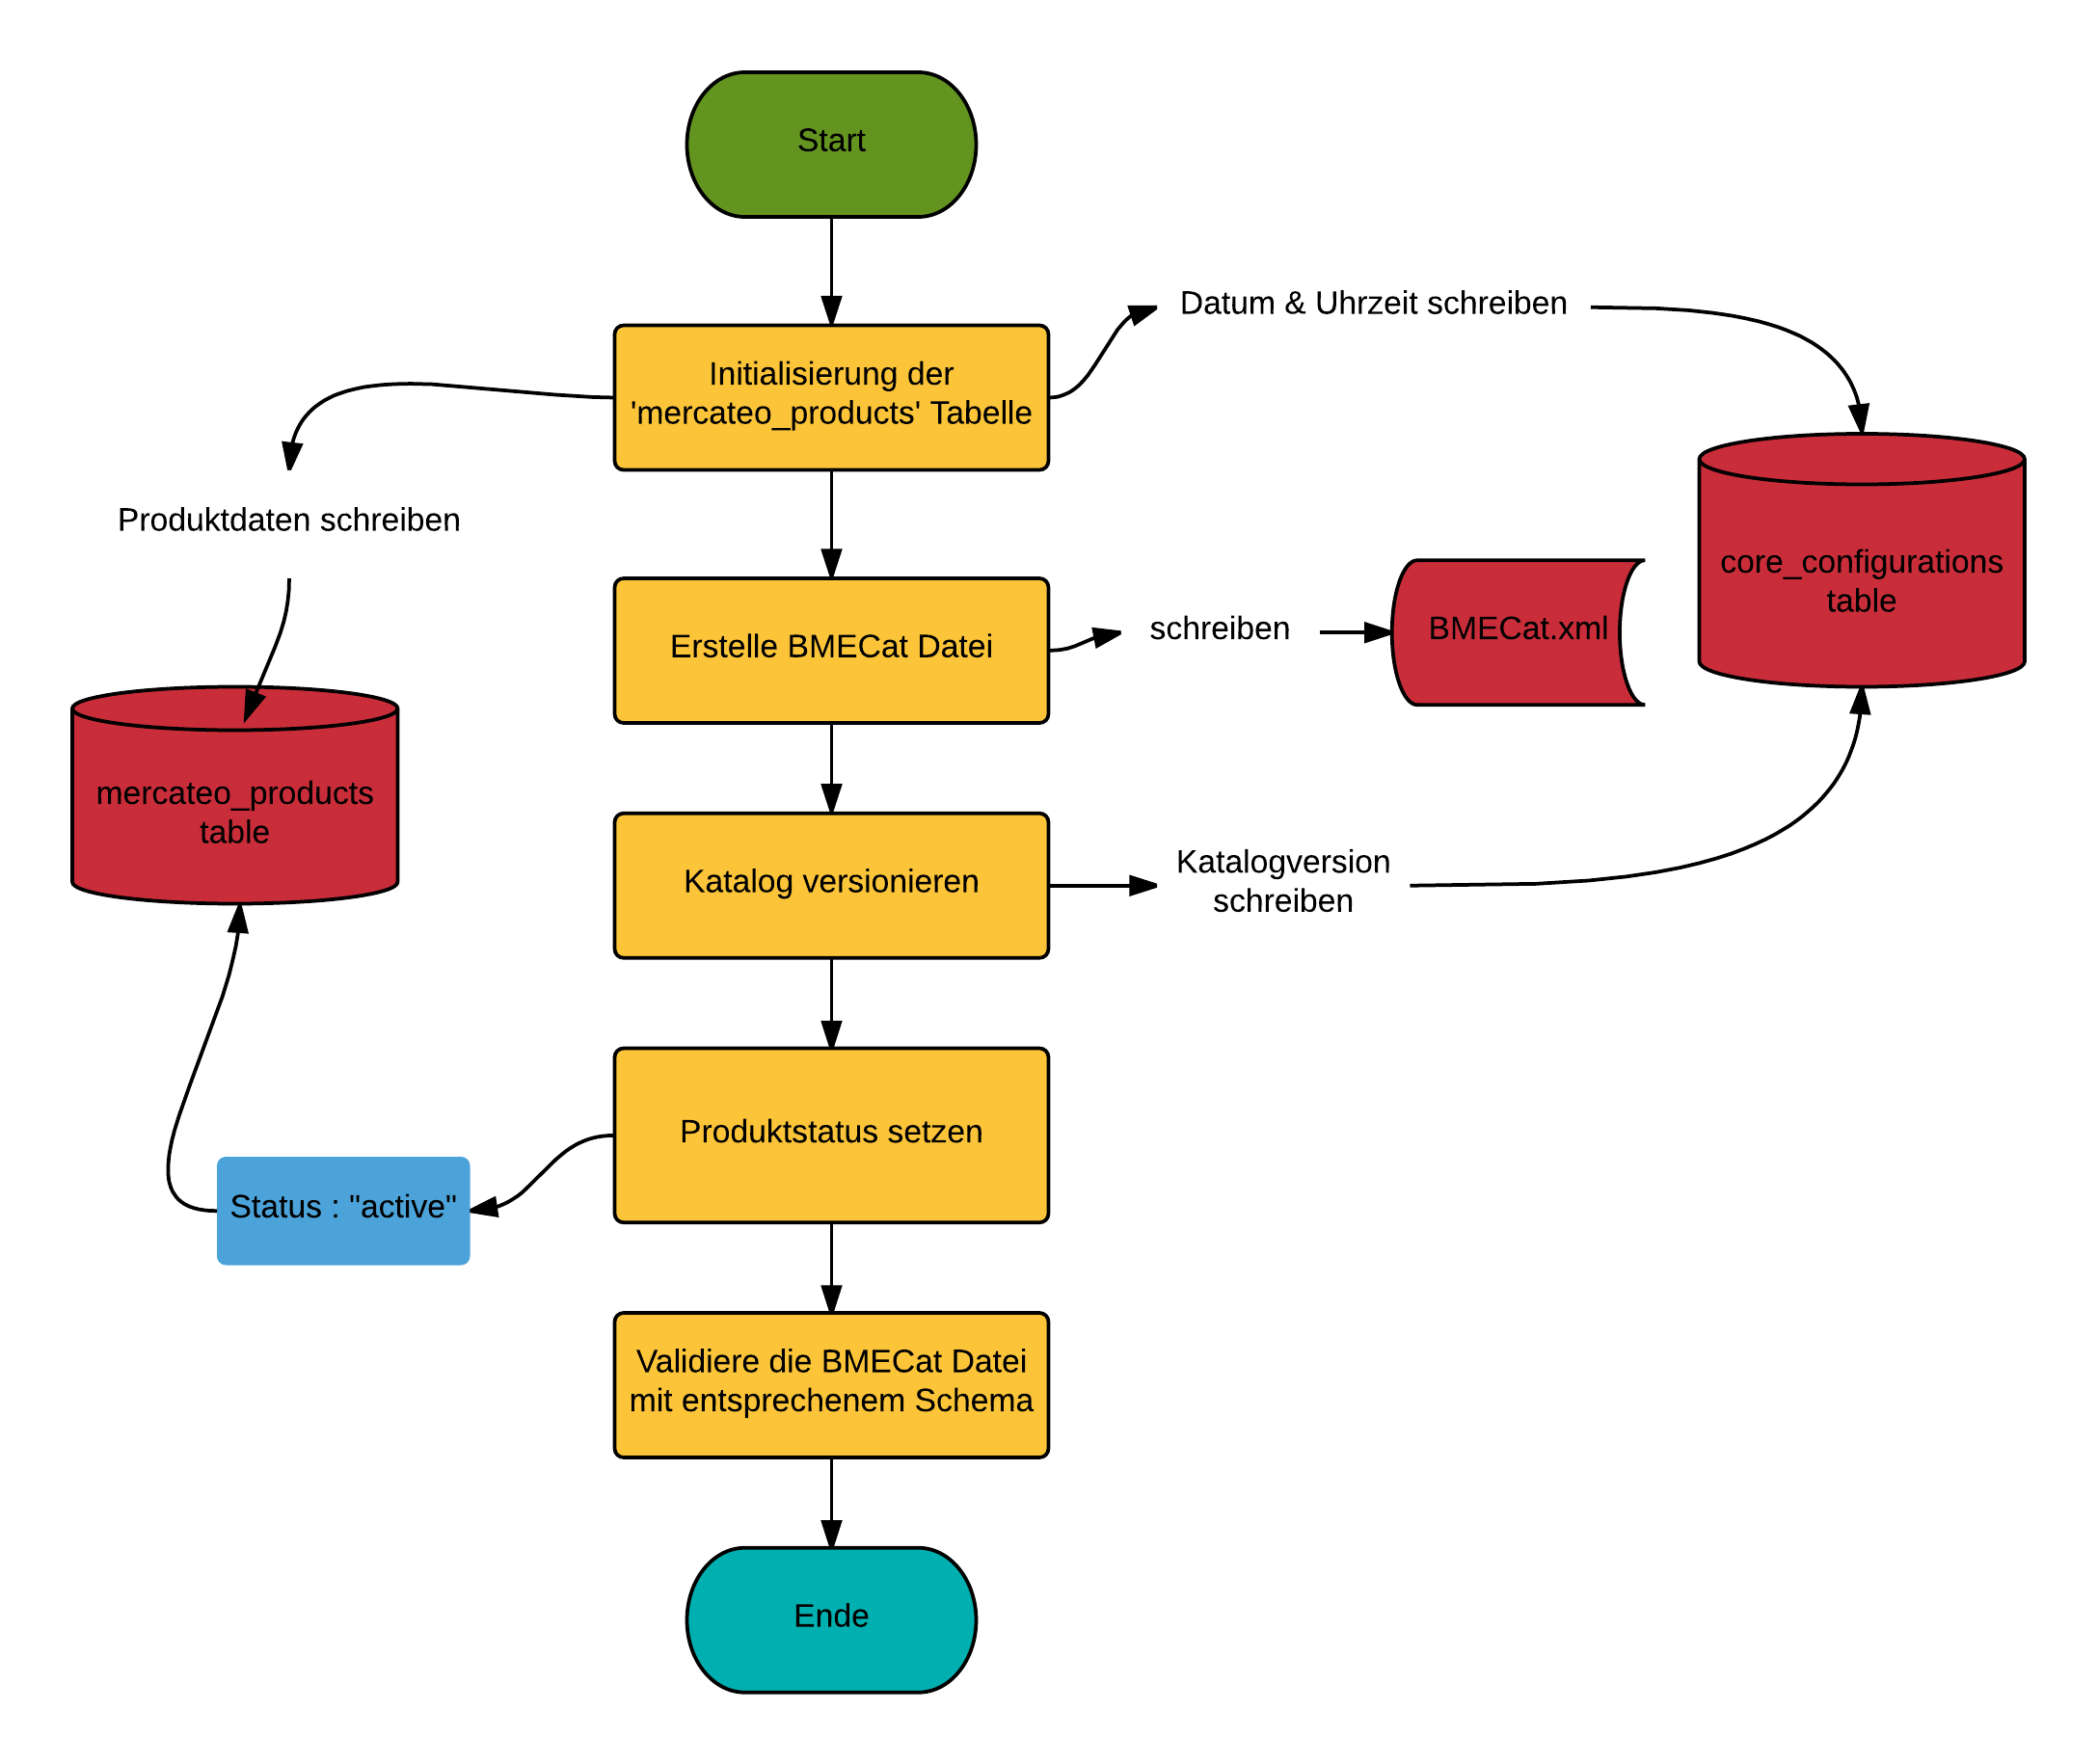
\includegraphics[width=0.7 \linewidth]{img/newCatalogFlow}
		\captionof{figure}[BasicLogic]{Programmlogik  bei der Transaktion \texttt{T\_NEW\_CATALOG}}
		\vspace{1em}
	\end{minipage}\\
	
	Nachdem das Katalogdokument geschrieben wurde wird es mithilfe des  XSD-Schemas (\texttt{bmecat\_new\_catalog\_1\_2.xsd}) überprüft. 
		
	\subsubsection{Katalogerstellungslogik bei der Transaktion \texttt{T\_UPDATE\_PRODUCTS}}
	
	Bei jedem erneuten Aufruf des Programmes wird zunächst überprüft ob Einträge in der \texttt{core\_products} Tabelle gelöscht, neu hinzugefügt oder geändert wurden. Letzteres geschieht mit Hilfe der Tabelle \texttt{core\_product\_updates} in der jede Änderung an einem \texttt{core\_product} mit dem Zeitstempel der Änderung erfasst wird. Ist einer der Fälle eingetreten wird der Status des Eintrages in der \texttt{mercateo\_products} Tabelle entsprechend gesetzt.
	
	\begin{minipage}{\linewidth}
		\vspace{1em}
		\centering
		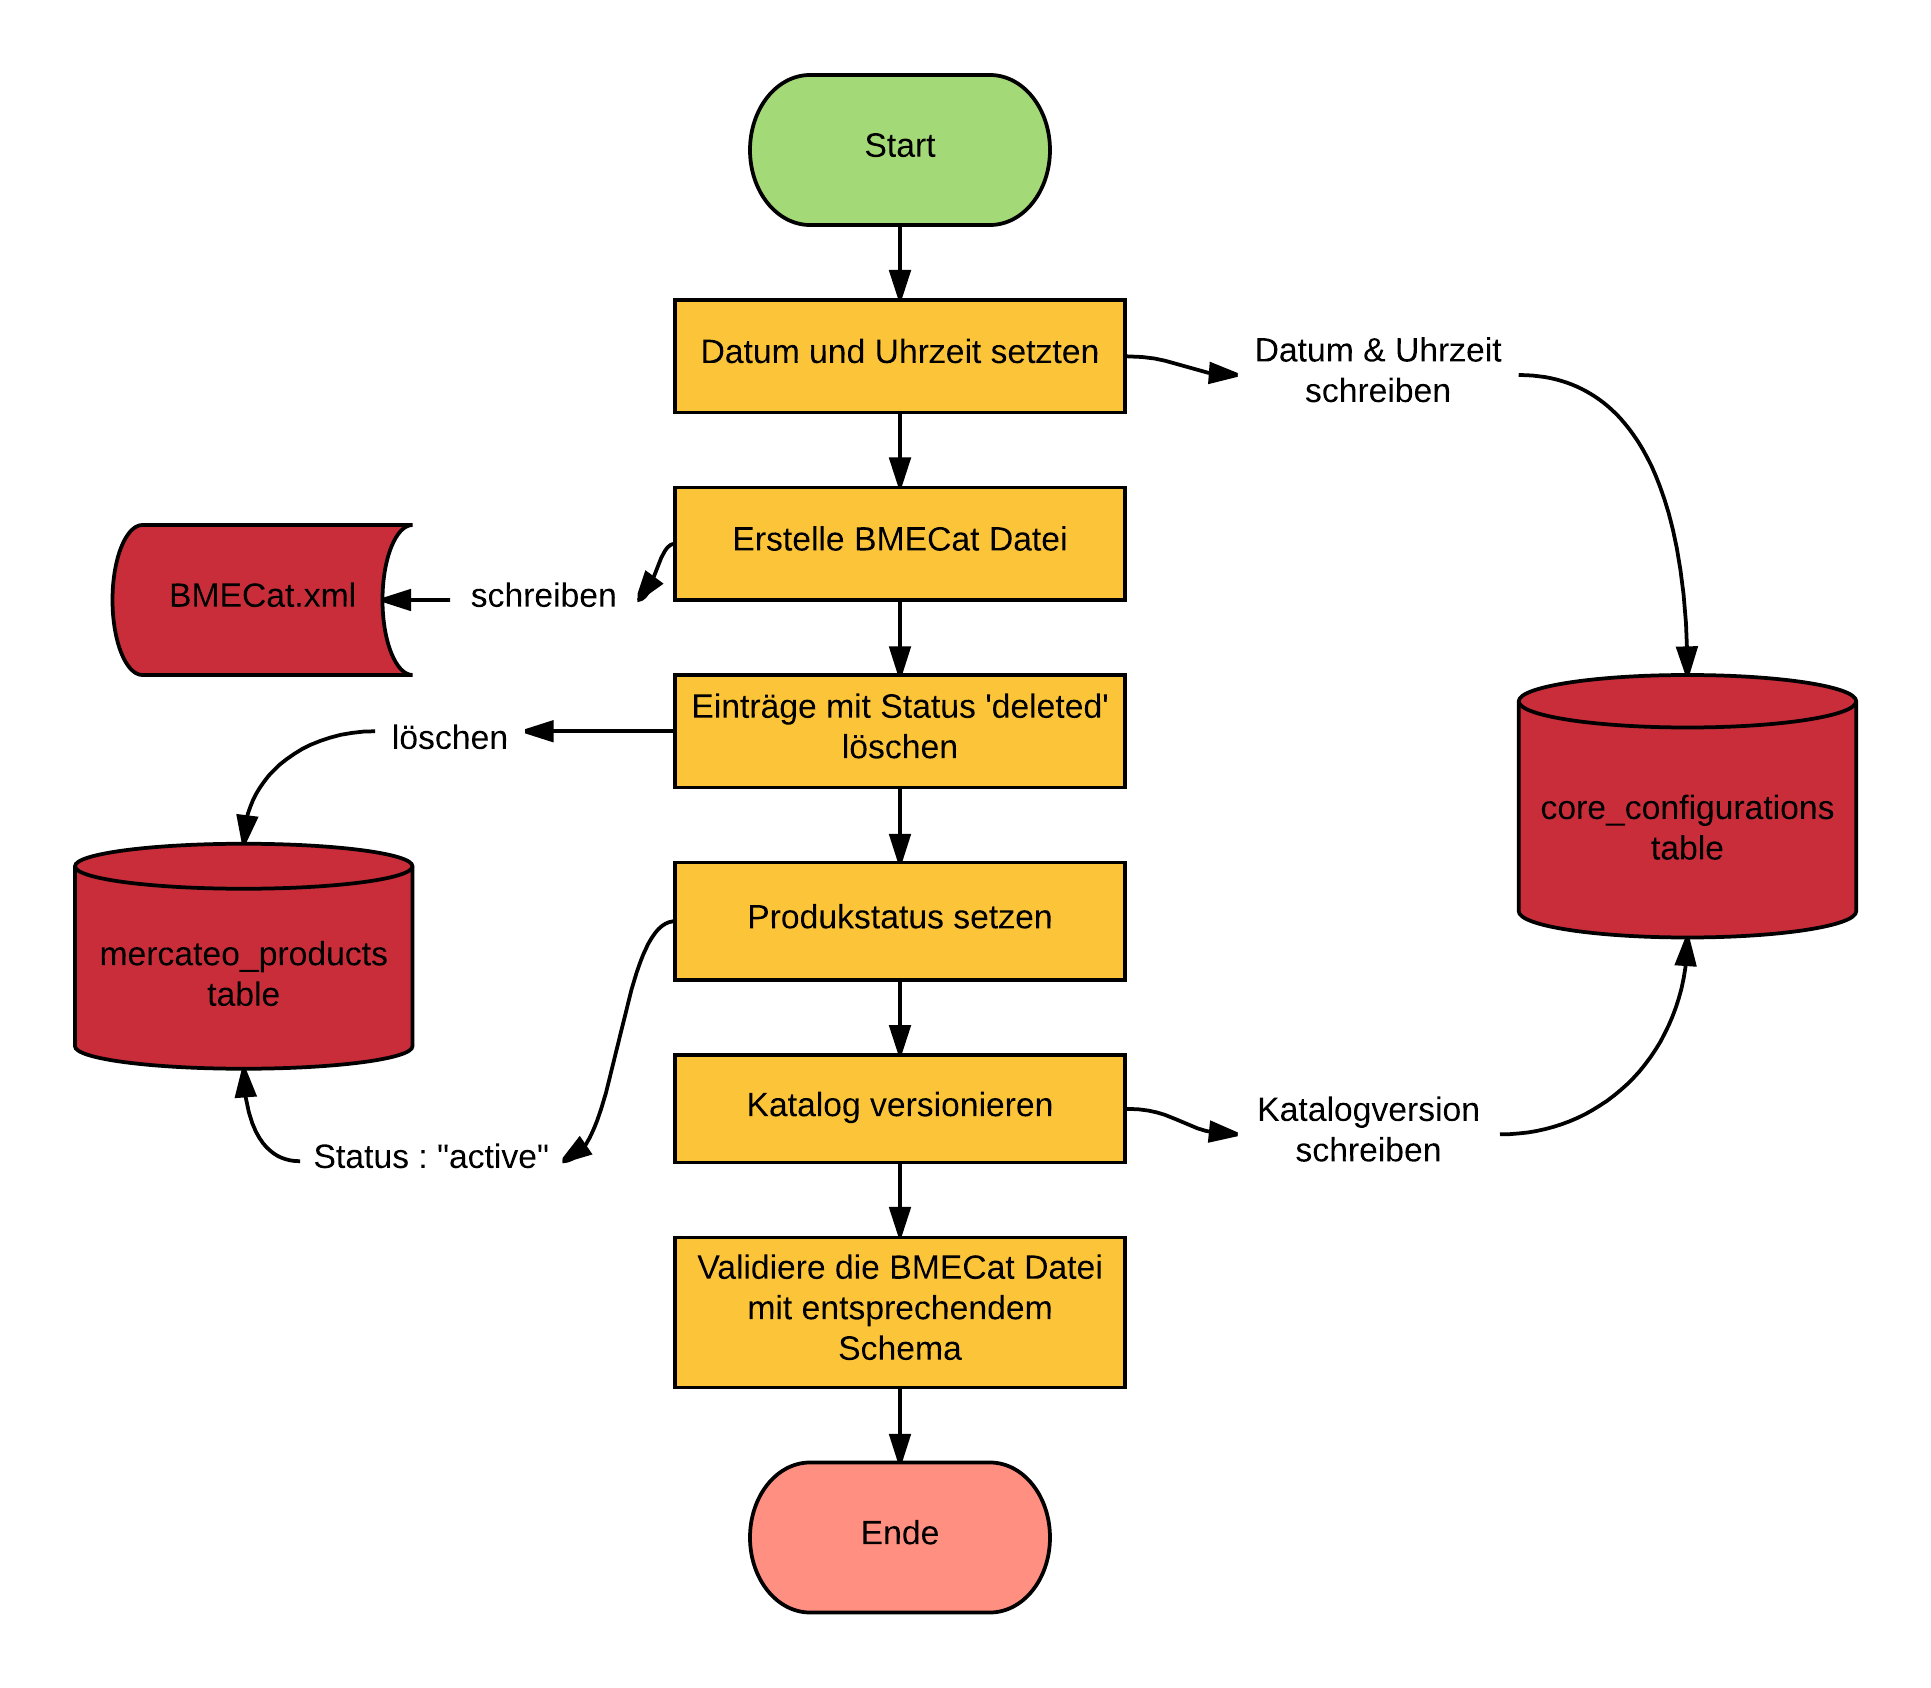
\includegraphics[width=0.7 \linewidth]{img/updateCatalogFlow}
		\captionof{figure}[BasicLogic]{Programmlogik  bei der Transaktion \texttt{T\_UPDATE\_PRODUCTS}}
		\vspace{1em}
	\end{minipage}\\
	
	
	Anschließend werden wiederum Datum \& Uhrzeit der Erstellung des Katalogdokumentes gesetzt und selbiges erstellt. Jene Einträge in \texttt{mercateo\_products}, die den Status \texttt{delete} haben, werden gelöscht, danach wird der Status der Übrigen auf \texttt{active} gesetzt und das Attribut \texttt{prev\_version} des Elementes \texttt{T\_UPDATE\_PRODUCTS} mit dem initialen Wert von '0' in die \texttt{core\_configurations} Tabelle geschrieben. Dieser Wert wird bei jedem Updatevorgang um '1' erhöht.	Abschließend erfolgt die Validierung des Dokumentes mithilfe des Schemas \texttt{bmecat\_update\_products\_1\_2.xsd}.
	
	\subsection{Bestandsdatenabfrage}
	
	Die Bestandsdatenabfrage wird mit einem einfachen Controller realisiert dessen \texttt{index()} Funktion als Parameter die angefragte SKU hat.
	Von Seiten Mercateo kann so eine URL der Form \url{http://itool.local/mercateo/availability/12} aufgerufen werden. Ist die SKU System vorhanden, wird die Bestandsmenge als Integer Wert zurückgeliefert, ist die angefragte SKU nicht im System, wird eine Fehlermeldung ausgegeben.
	
	\section{Implementierung}
	
	Die Implementierung gliedert sich in 2 Bereiche, die Konsolenanwendung zur Generierung des Katalogdokumentes und die Bestandsdatenabfrage.
	
	\subsection{Die BMECat Creator Shell}
	
	Mit der BMECat Creator Shell wird der Entwurf zur Erzeugung eine BMECat Katalogdokumentes umgesetzt. Die eigentliche Shell Klasse \texttt{BmeCatCreatorShell} dient in der Implementierung nur dazu das Subcommando \texttt{prepareCatalogTask} aufzurufen und sicherzustellen, dass die notwendigen Argumente übergeben werden.
	\lstset{basicstyle=\scriptsize\ttfamily}
	\begin{lstlisting}
	Usage:
	cake mercateo.bme_cat_creator [subcommand] [-h] [-q] [-v] <Core Seller Id> [<Delete flag>]
	Subcommands:
	prepareCatalog  Creates or updates a BMECat Catalog file.
	
	To see help on a subcommand use `cake mercateo.bme_cat_creator [subcommand] --help`
	
	Options:	
	--help, -h     Display this help.
	--quiet, -q    Enable quiet output.
	--verbose, -v  Enable verbose output.
	
	Arguments:	
	Core Seller Id  The ID of the Seller for whom the BMECat shall be
	                created
	Delete flag     If "del" is set as second Argument, the
	                mercateo_products table will be truncated
	                (optional)
	\end{lstlisting}
	
	Dabei liegt dem Programm folgende Aufrufhierarchie zugrunde:\\
	\begin{minipage}{\linewidth}
		\vspace{1em}
		\centering
		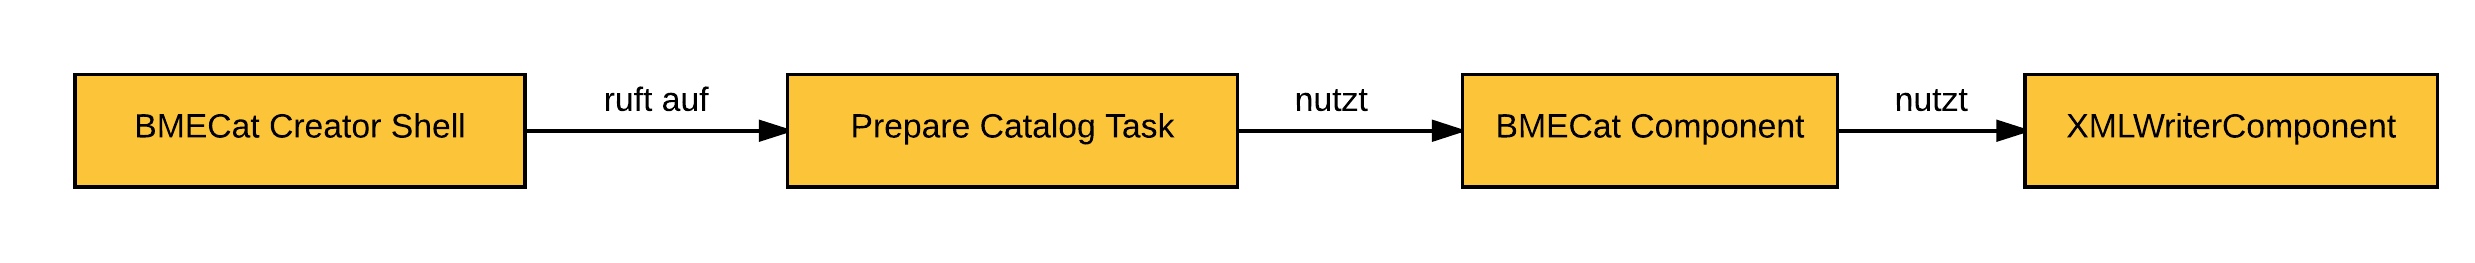
\includegraphics[width=1 \linewidth]{img/shellFlow}
		\captionof{figure}[BasicLogic]{Aufrufhierarchie BMECatCreatorShell}
		\vspace{1em}
	\end{minipage}\\
	
	Im Folgenden werden die einzelnen Klassen vorgestellt.
	
	\subsection{XMLWriterComponent}
	
	Die XMLWriterComponent Klasse ist insofern wichtiger Bestandteil der Implementierung, als das ohne sie nur auf umständlicherem Wege XML geschrieben werden kann. Hier seien nun in Kürze jene Methoden vorgestellt, die von der Klasse BMECatComponent genutzt werden:
	
	\begin{enumerate}[noitemsep]
	\item public function openXmlWriter($filePath, $rootElement, $attributes = null, $doctype = null) \\
		  Ermöglicht das Anlegen einer neuen XML Datei mit der Option Attribute ( z.B. die BMECat Version) zu übergeben, sowie über den DOCTYPE eine entsprechende .dtd Datei zu referenzieren.
	\item public function closeXmlWriter() \\
		  Schließt das XML Dokument ab.
	\item writeXmlElement($name, $value, $type = "text", $attributes = [])\\
		  Schreibt ein XML Element mit dem übergebenen Wert und den dazugehörigen Attributen und schließt es sogleich ab. (Schreibt Start- und End Tag)
	\item public function writeStartXmlElement($name, $attributes = [])\\
		  Öffnet ein XML Element und setzt die übergebenen Attribute. (Schreibt den Start-Tag)
	\item public function writeEndXmlElement()\\
		  Schließt das zuvor geöffnete Element ab. (Schreibt den End-Tag)
	\end{enumerate}
	
	VORTEILE? 
	
	\subsection{BMECatComponent}
	
	Die Klasse BMECatComponent dient dazu ein wohlgeformtes und gültiges XML Dokument entsprechend den BMECat- und Mercateo Vorgaben zu erstellen. Wie im Kapitel Grundlagen bereits beschrieben gliedert sich ein BMECat Dokument in 4 Bereiche und zwar den Header, das Kataloggruppensystem, die Auflistung der einzelnen Artikel und die Zuordnung der Artikel zu ihren Kategorien. Der BMECat Komponent stellt für jeden dieser Teilbereiche Funktionen bereit die in Folge erläutert werden sollen.
	Zur Orientierung dient eine Übersicht der Aufrufhierarchie.\\
	
	\begin{minipage}{\linewidth}
		\vspace{1em}
		\centering
		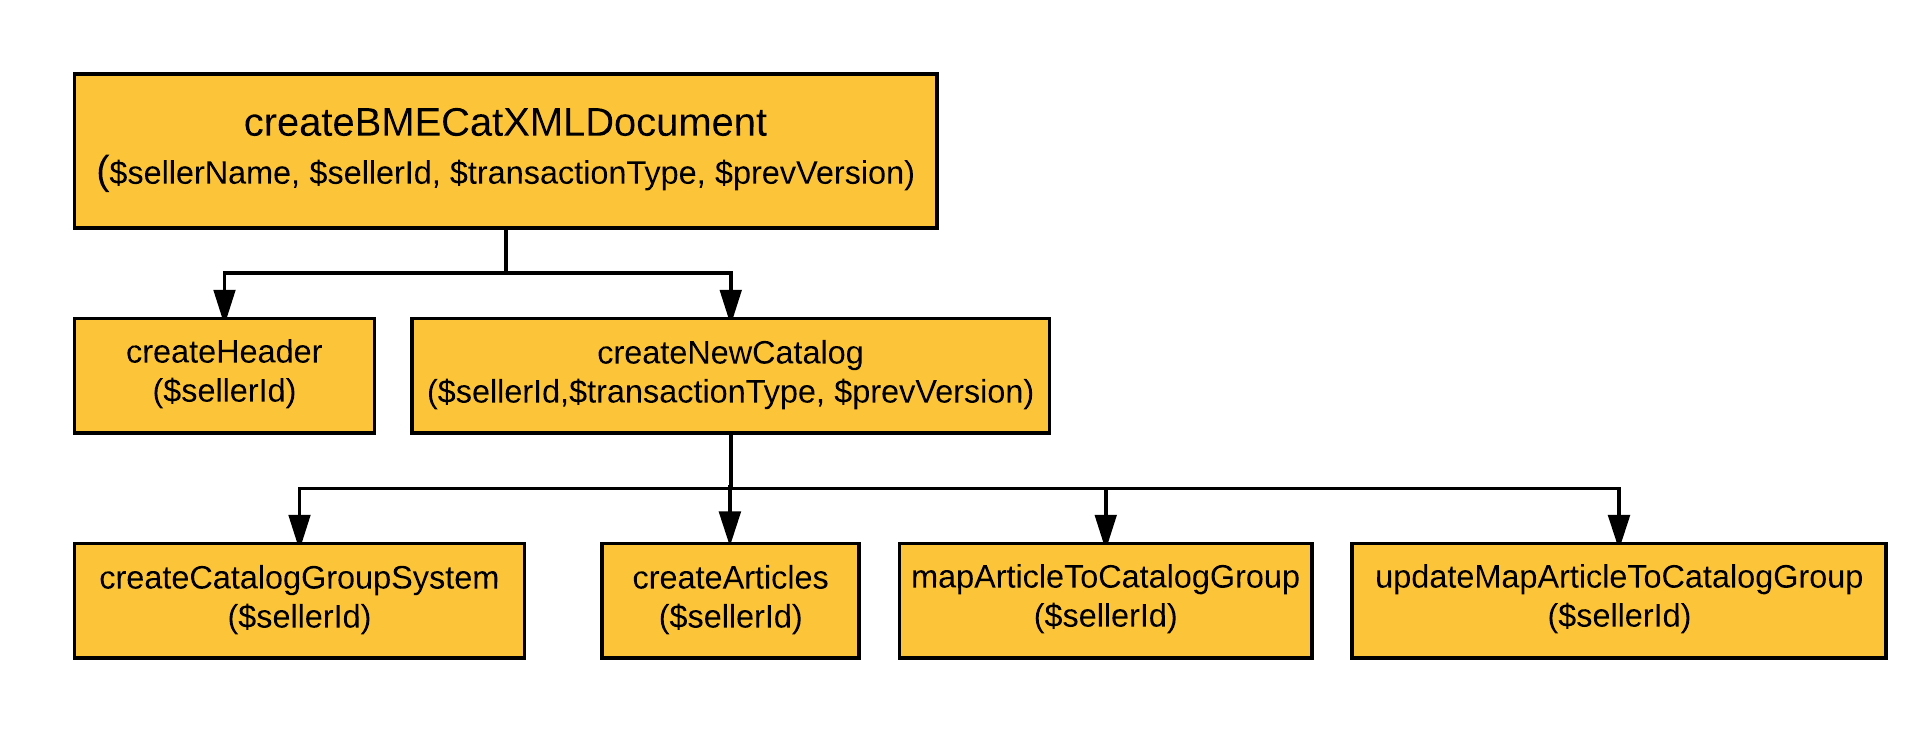
\includegraphics[width=0.7 \linewidth]{img/createBMECatHierarchie}
		\captionof{figure}[BasicLogic]{Aufrufhierarchie createBMECatXMLDocument}
		\vspace{1em}
	\end{minipage}
	
	
	
	
	
	\subsubsection{Erstellen des BMECat Dokumentes}
	
	Die Funktion \texttt{createBMECatXMLDocument(\$sellerName, \$sellerId, \$transactionType, \$prevVersion)} dient der Erzeugung eines BMECat Dokumentes. Sie legt die die XML Datei mit der Namenskonvention \texttt{'Verkäufername\_Erzeugungsdatum\_Erzeugungszeit.xml'} an und schreibt Informationen zum XML Namensraum (xmlns) und zur Dokumenttypdefinition (dtd) in die XML-Deklaration. Von ihr werden die Methoden zur Erzeugung des Headers und der restlichen Abschnitte des BMECat Dokumentes aufgerufen.
	Anhand des Parameters \texttt{\$transactionType} wird entschieden ob bei dem zu erzeugenden Dokument die Transaktion \texttt{T\_NEW\_CATALOG} oder \texttt{T\_UPDATE\_PRODUCTS} umgesetzt werden soll.
	
	\subsubsection{Schreiben der Header Sektion}

	Die Methode \texttt{createHeader(\$sellerId)} schreibt die BMECat-Header-Sektion des Dokumentes. Alle benötigten Informationen, wie z.B. Herstellername oder Katalogversion werden dabei anhand der \texttt{sellerId} aus der \texttt{mercate\_accounts} Tabelle geladen.
	
	\subsubsection{Schreiben des Kataloggruppensystems}
	
	Die Methode \texttt{createCatalogGroupSystem(\$sellerId)} steuert die Erzeugung des Kataloggruppensystems. Die von ihr aufgerufenen Methoden sind im wesentlichen für das Schreiben bestimmter XML Elemente zuständig.\\
	\begin{minipage}{\linewidth}
		\vspace{1em}
		\centering
		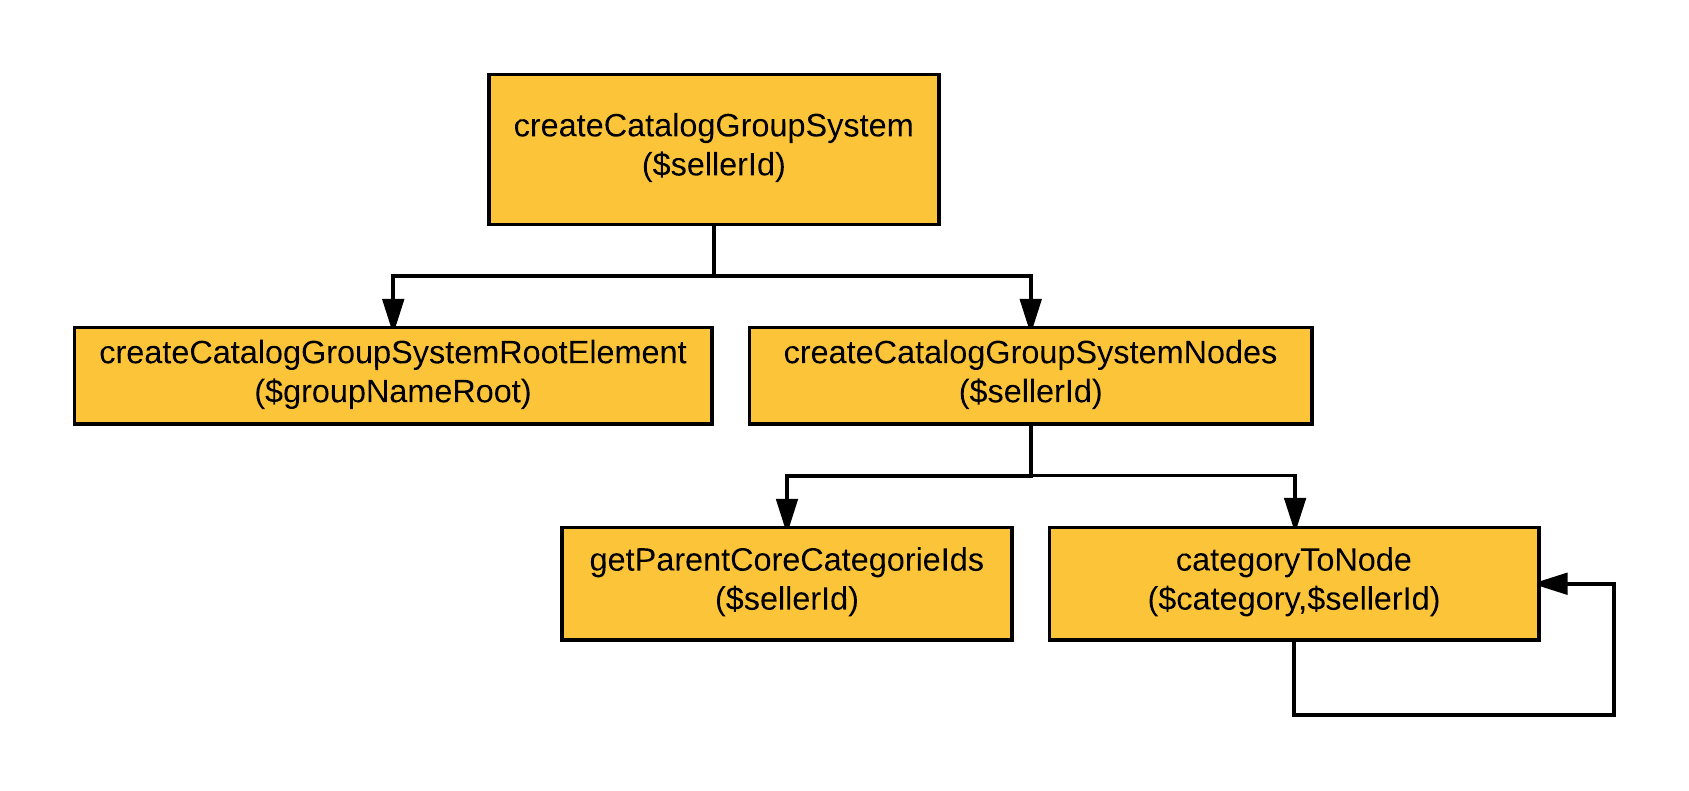
\includegraphics[width=0.7 \linewidth]{img/CreateCatalogGroupSystemHierarchie}
		\captionof{figure}[BasicLogic]{Aufrufhierarchie createCatalogGroupSystem}
		\vspace{1em}
	\end{minipage}
	
	 Das tatsächliche Abbilden der Katalogstruktur erfolgt in der Methode \texttt{categoryToNode(\ \$category,\$sellerId)}.
	 
	\begin{addmargin}[1cm]{1cm}
	\underline{Dazu ein kleiner Exkurs:}\\
		 CakePHP bietet die Möglichkeit einem Model ein sogenanntes Tree-Behaviour hinzuzufügen. Dieses basiert auf dem Nested-Set-Konzept, das es ermöglicht hierarchische Strukturen in relationalen Datenbanken abzubilden\footnote{vgl. hierzu\url{https://www.sitepoint.com/hierarchical-data-database-2/}}. Die \texttt{core\_categories} Tabelle bedient sich dieses 'Behavious', was es ermöglicht diesen Kategoriebaum rekursiv zu durchlaufen und dadurch das Kataloggruppensystem des BMECat abzubilden.
	\end{addmargin}
	
	
	Die Methode \texttt{categoryToNode(\$category,\$sellerId)} durchläuft, ausgehend vom Wurzelelement, alle Kindelemente und schreibt die entsprechenden Daten in das Dokument. Solange dabei die Anzahl der Kindelemente des gerade traversierten Elementes größer 0 ist wird dabei dem Attribut \texttt{type} der Wert \texttt{node} zugewiesen. Gibt es keine Kindelemente mehr, wird der Wert auf \texttt{leaf} gesetzt. 
	\lstset{language=xml}
	\begin{lstlisting}
	<CATALOG_STRUCTURE type="node">
	 <GROUP_ID>207</GROUP_ID>
	 <GROUP_NAME>Auto -Motorrad - Flugzeug</GROUP_NAME>
	 <PARENT_ID>202</PARENT_ID>
	</CATALOG_STRUCTURE>
	<CATALOG_STRUCTURE type="leaf">
	 <GROUP_ID>210</GROUP_ID>
	 <GROUP_NAME>Oldtimer</GROUP_NAME>
	 <PARENT_ID>207</PARENT_ID>
	</CATALOG_STRUCTURE>
	\end{lstlisting}
	
	\subsubsection{Artikelerstellung}
	
	Die Methode \texttt{createArticles(\$sellerId)} aggregiert die zu schreibenenden Artikeldaten. Über einen \texttt{INNER JOIN} werden die Tabellen \texttt{mercateo\_products} und \texttt{core\_products} verbunden, so dass über die in \texttt{mercateo\_products} hinterlegte \texttt{core\_product\_id} die entsprechenden Daten aus der \texttt{core\_products} Tabelle nachgeladen werden können. 
	Ist der Artikelstatus gleich \textit{'new'} oder \textit{'update'} wird die Methode \texttt{writeArticle(\$product, \$articleMode)} aufgerufen, die die entsprechenden XML Elemente schreibt. \\
		
		\begin{minipage}{\linewidth}
			\vspace{1em}
			\centering
			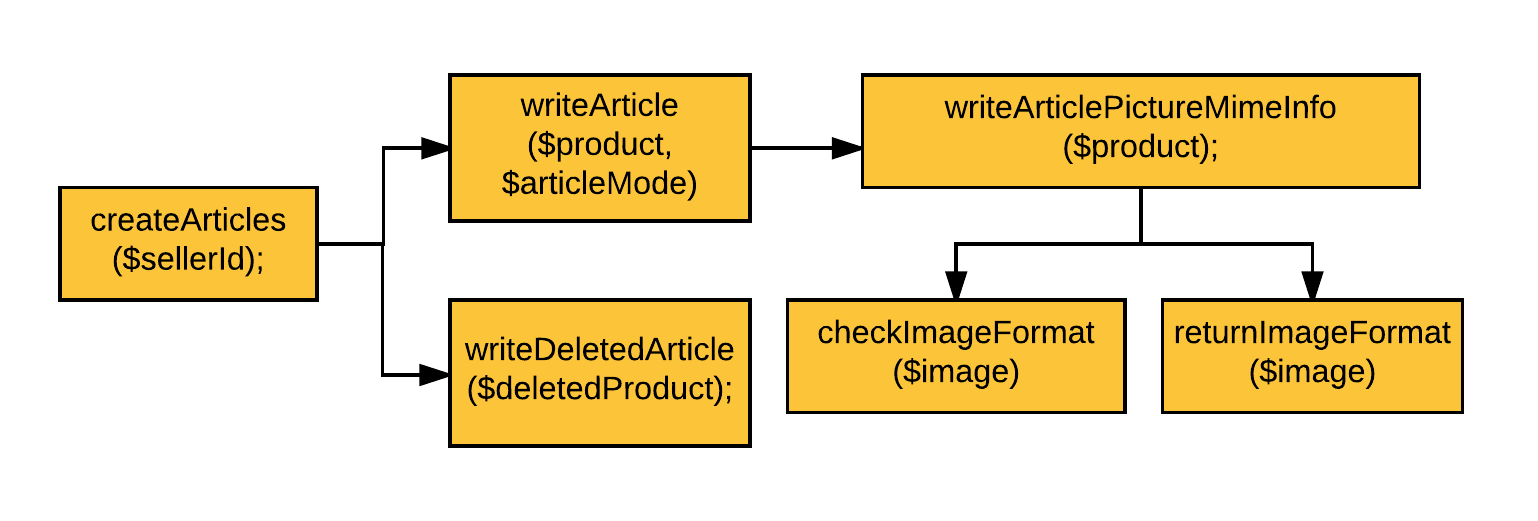
\includegraphics[width=0.7 \linewidth]{img/createArticleHierarchie}
			\captionof{figure}[BasicLogic]{Aufrufhierarchie createArticle}
			\vspace{1em}
		\end{minipage}
	
	Zusätzlich wird geprüft ob die dem Artikel zugeordneten Bilder der Mercateo Spezifikation entsprechen. Diese gestattet als Bildformate nur '.jpeg' und '.png'. Entsprechen die Bilddateien nicht diesem Format wird eine entsprechende Ausnahmebehandlung durchgeführt. Dabei wird der komplette Pfad der beanstandeten Datei zurückgeliefert, um es dem Anwender zu erleichtern diesen Fehler zu beheben.\\
	
	\begin{lstlisting}
	2017-01-05 16:30:55 Info: Product with CoreProductId: 7147 updated
	Exception: 'png' ist not allowed as File Extension.
	Only .gif & .jpg Files are accepted by Mercateo-Marketplace
	Check Image Path: https://bild-im-rahmen.com/wp-content/uploads/2016/03/s21r.png
	\end{lstlisting}

	Handelt es sich um einen gelöschten Artikel, wird die Methode \texttt{writeDeletedArticle(\$pro\-duct)} aufgerufen. Diese schreibt die in \texttt{mercateo\_products} hinterlegten, um einen Artikel als gelöscht auszeichnen zu können notwendigen Informationen - Die SKU \& den Titel- in das Dokument.
	
	\subsubsection{Kategoriemapping}
	
	Mit der Methode \texttt{mapArticleToCatalogGroup(\$sellerId)} werden bei der Transaktion \texttt{T\_NEW\_CATALOG} die Artikel ihren Kategorien zugewiesen. Alle dazu notwendigen Informationen finden sich in der \texttt{mercateo\_products} Tabelle.
	
	Wird ein Update Katalog erstellt wird die Funktion \texttt{updateMapArticleToCatalogGroup()} aufgerufen. Sie setzt den bei der Transaktion \texttt{T\_UPDATE\_PRODCUTS} geforderten Attributwert für \texttt{mode} entsprechend der Angaben in der \texttt{mercateo\_products} Tabelle.
	Mögliche Werte sind \textit{'new'} für neu erstellte und \textit{'delete'} für gelöschte Produkte.
	
	
	\section{prepareCatalogTask}
	
	

	
	
	
	
	
	
	
	
	
	
	
	
	
	
	
	
	
	
	
	
	
	
	
	
	
	
	
	
	
	
	
	
	

	
	\section{Test}

	Hier kann vielleicht auch die Validation rein (MercateoAccountsTable)
	

